%================================================================================
%       Safety Critical Systems Club - Data Safety Initiative Working Group
%================================================================================ 
%                       DDDD    SSSS  IIIII  W   W   GGGG
%                       D   D  S        I    W   W  G   
%                       D   D   SSS     I    W W W  G  GG
%                       D   D      S    I    WW WW  G   G
%                       DDDD   SSSS   IIIII  W   W   GGG
%================================================================================
%               Data Safety Guidance Document - LaTeX Source File
%================================================================================
%
% Description:
%   This is the main document file, it simply marks the beginning and end of the
%   document and 'includes' each of the document sections, in the required order.
%
% Notes:
%   All of the actual document content is contained within each of the files
%   that are 'included' by this one.
%
%================================================================================
%================================================================================
% Configuration for different versions of the document
%================================================================================

% Comment out the options that are not wanted
% The version for printing should have all four options disabled

\def\withCovers{}
\def\withBlueHyperlinks{}
\def\withChangebars{} %Markers are \cbstart and \cbend. Remember to delete markers for previous changes before starting update.
\def\withToDo{} %Post-it note in the margin to highlight issues to be resolved before publication

%Load the template containing all of the style for the doc
%================================================================================
%       Safety Critical Systems Club - Data Safety Initiative Working Group
%================================================================================
%                       DDDD    SSSS  IIIII  W   W   GGGG
%                       D   D  S        I    W   W  G   
%                       D   D   SSS     I    W W W  G  GG
%                       D   D      S    I    WW WW  G   G
%                       DDDD   SSSS   IIIII  W   W   GGG
%================================================================================
%               Data Safety Guidance Document - LaTeX Source File
%================================================================================
%
% Description:
%   This file contains all of the LaTeX macros to control the template for the
%   Data Safety Guidance Document.
%
% !!WARNING!!
%   CHANGING THE CONTENT OF THIS PARTICULAR FILE CAN SERIOUSLY AFFECT THE
%   APPEARANCE AND LAYOUT OF THE GENERATED DOCUMENT, SO PLEASE BE CAREFUL.
%
% Label formats:
%   bkm: ==>      Reference to another part of this document
%   citation: ==> Reference to an external document listed in bibTex
%   fig: ==>      Reference to a figure within this document
%   ftn: ==>      Reference to a footnote within this document
%   tab: ==>      Reference to a table within this document
%
% Notes:
%   All commands, styles, colours, etc. defined within this template shall begin
%   with the prefix of 'dsiwg' to distinguish them from built-in TeX keywords or
%   those in third-party packages.
%

%================================================================================
%Version 2.0 was US Letter paper with a default font of 10pt, this may change
%================================================================================
\documentclass[letterpaper,10pt,twoside]{article}

% May be able to remove in future, when pdflatex default output becomes pdf 1.7 or greater
\pdfminorversion=7 % Required to read darkknowns.pdf at v1.7, but default from pdflatex is 1.5

%================================================================================
%Set the default font family and series for the document to 'Open Sans Light'
%================================================================================
\usepackage[utf8]{inputenc}
\usepackage[T1]{fontenc}
\usepackage[default,defaultsans]{opensans}% On TeXLive 2018, "default" was enough. Need "defaultsans" from TeXLive 2019
\usepackage{textcomp}           %Required for complete font support
\renewcommand{\seriesdefault}{l}% Select Open Sans Light as the default font

%================================================================================
%Load all other required packages
%================================================================================
\usepackage[
  title,%
  titletoc%
]{appendix}                     %Used to add appendices into the ToC
\usepackage{tocvsec2}           %Allow suppression of selected entries within TOC
%--------------------------------------------------------------------------------
\usepackage{calc}               %Used for infix calculations, e.g. column widths 
\usepackage{color}              %Used to set foreground and background colours
\usepackage{colortbl}           %Used to add colour to LaTeX tables
\usepackage{enumitem}           %Used to control the different list environments
\usepackage{fancyhdr}           %Used to define the header and footer layout
\usepackage{float}              %Used to force specific placement of images
\usepackage[hang]{footmisc}     %Used to make footnotes a numbered list
%--------------------------------------------------------------------------------
\ifx\withChangebars\undefined
% Shortcut to create version without changebars
\newcommand{\cbstart}{}
\newcommand{\cbend}{}
\else
\usepackage{changebar}          %Markers are \cbstart and \cbend.
\fi
%--------------------------------------------------------------------------------
\usepackage[
  dvips =false,%
  pdftex=false,%
  vtex  =false,%
  bottom=1.5cm,%
  left  =2.5cm,%
  right =2.5cm,%
  top   =1.5cm,%
  head  =18pt  %
]{geometry}                     %Used to set-up the page layout and margins
%--------------------------------------------------------------------------------
\usepackage[pdftex]{graphicx}   %Used to insert diagrams into the document
%--------------------------------------------------------------------------------
%\usepackage[
%  acronyms,%
%  toc
%]{glossaries}                   %Used to create and print the glossary - very sensitive to package order
%--------------------------------------------------------------------------------
\usepackage[none]{hyphenat}     %Used to prevent hyphenation in the document
\usepackage{longtable}          %Used for tables that break across pages
\usepackage{caption}            %Adds longtable* which is needed to create longtables that do not increment the table counter
\usepackage{multirow}           %Used to allow multiple row spanning in tables
\usepackage{pifont}             %Used to print ZipfDingbats characters (\ding)
\usepackage[many]{tcolorbox}    %Used to place coloured boxes around text

\ifx\withToDo\undefined
% Shortcut to create version without todo notes
\newcommand{\todo}[1]{}
\newcommand{\listoftodos}{}
\else
\usepackage[textwidth=2cm]{todonotes} %Allows multi-line markup of text which needs to be amended/reviewed ie, yellow highlighter
\fi

\usepackage{pdfpages}           %Handy way to insert covers
\usepackage{wrapfig}            %Wrap text around a figure
\usepackage{imakeidx}

\usepackage[framemethod=tikz]{mdframed}           %Put text in a box that can break across pages
\newmdenv[frametitle=Response of the AI,%
  roundcorner=10pt,
linewidth=2pt]{aibox} % Environment to display AI-generated text
%--------------------------------------------------------------------------------
% Set up indexes.
% Page style gets upset for indexes, unless we set it explicitly
%
\makeindex[name=locationidx,title=Index of Locations,intoc]
\makeindex[title=Index,intoc]
\indexsetup{
  othercode={%
    \thispagestyle{Standard}%
  }
}
% Break long URLs
\usepackage{url}
\def\UrlBreaks{\do\/\do-}
\usepackage{breakurl}
%--------------------------------------------------------------------------------
%The hyperref is best loaded last to avoid conflicts, e.g. with glossaries
%TGR: the glossaries package documentation says it must be loaded after the hyperref package.
%--------------------------------------------------------------------------------
\ifx\withBlueHyperlinks\undefined
\usepackage[                    %Could use \hypersetup but easier to do it here
  breaklinks,%
  bookmarksnumbered,%
  pdftex,%
  pdfpagelayout=OneColumn,% "OneColumn" produces a single continous scrolling viewer display; was previously set to "TwoColumnRight" for two pages side by side with odd pages on the right.
  pdfpagelabels,%
  hidelinks,% Make the links visually just normal text
  linktoc=page
]{hyperref}                     %Creates property fields & hyperlinks in the PDF - For details see http://www.tug.org/applications/hyperref/manual.html#x1-110003.7
\else
\usepackage[                    %Could use \hypersetup but easier to do it here
  bookmarksnumbered,%
  pdftex,%
  pdfpagelayout=OneColumn,% "OneColumn" produces a single continous scrolling viewer display; was previously set to "TwoColumnRight" for two pages side by side with odd pages on the right.
  pdfpagelabels,%
  colorlinks=true,% Select coloured text, rather than coloured boxes around links
  linkcolor=blue,          % color of internal links (change box color with linkbordercolor)
  citecolor=blue,        % color of links to bibliography
  filecolor=blue,      % color of file links
  urlcolor=blue,           % color of external links
  linktoc=page
]{hyperref}                     %Creates property fields & hyperlinks in the PDF - For details see http://www.tug.org/applications/hyperref/manual.html#x1-110003.7
\fi

%================================================================================
%Create some new commands to quickly change local font style
%================================================================================
\DeclareRobustCommand\ebseries{\fontseries{eb}\selectfont}
\DeclareRobustCommand\sbseries{\fontseries{sb}\selectfont}
\DeclareRobustCommand\ltseries{\fontseries{l}\selectfont}
\DeclareRobustCommand\clseries{\fontseries{cl}\selectfont}
\DeclareRobustCommand\regseries{\fontseries{m}\selectfont}

\DeclareTextFontCommand{\dsiwgTextEB}{\ebseries}    %Extra-Bold typeface
\DeclareTextFontCommand{\dsiwgTextSB}{\sbseries}    %Semi-Bold typeface
\DeclareTextFontCommand{\dsiwgTextLT}{\ltseries}    %Light typeface
\DeclareTextFontCommand{\dsiwgTextCL}{\clseries}    %Condensed-light typeface
\DeclareTextFontCommand{\dsiwgTextREG}{\regseries}  %Regular typeface

\DeclareTextFontCommand{\dsiwgTextBF}{\sbseries}    %What 'bold-face' looks like
\DeclareTextFontCommand{\dsiwgTextIT}{\itshape}     %What 'italic' looks like

%
%Create a new environment to change the font shape for large blocks of text.
%Using begin/end is more obvious than just using one of the above commands.
%
\newenvironment{dsiwgBold}{\sbseries}{}
\newenvironment{dsiwgItalic}{\itshape}{}

%
%Unfortunately the Open Sans font doesn't support a typewriter style in 'light'
%series, so we have to declare a special version to avoid warnings when compiling
%the document.
%
% For manual use:
\newcommand{\dsiwgTextTT}[1]{\usefont{T1}{cmtt}{m}{n}{#1}}
%
% To make \url use the right font
% We need these next two lines, but they fail to load T1/cmtt/m/n, so we put up with warning for now
%\DeclareFontFamily{T1}{cmtt}{\hyphenchar\font=-1}
%\DeclareFontShape{T1}{cmtt}{l}{n}{ <-> ssub * cmtt/m/n }{}

%
%Set the character to be used for the check box on the ODR forms, etc.
%
\newcommand{\dsiwgCheckBox}{\large{\ding{111}}}

%================================================================================
%Space things out a bit
%================================================================================
\linespread{1.2}

%================================================================================
%Mark intentionally blank pages as such
%================================================================================
\makeatletter
\def\dsiwg@intblankpage{%
	\clearpage% this line has no effect if invoked from dsiwg@cleardoublepage
	\null\vfil
	\centerline{This page is intentionally blank}%
	\newpage
        \phantomsection% Required to move page counter in \label associated with following \section point to correct page
}

\def\dsiwg@cleardoublepage{%
    \clearpage%needed here so that we test AFTER the page throw
	\ifodd\c@page\else
		\dsiwg@intblankpage
	\fi
}
\let\cleardoublepage=\dsiwg@cleardoublepage
\makeatother

%================================================================================
%Define the colours to be used for this template style
%================================================================================
%
%Document accent colour for headings, etc. (set to a shade of blue)
%
%\definecolor{dsiwgAccentColour}{RGB}{233,33,33} %Red - v2.0
\definecolor{dsiwgAccentColour}{RGB}{0,102,255} %Blue - v3.0
\definecolor{dsiwgDimColour}{RGB}{51,153,255} %Pale Blue - v3.6
%
%Colours to be used for the objectives list box at the start of each section 
%
%\definecolor{dsiwgObjectiveBackgroundColour}{RGB}{233,15,12}
%\definecolor{dsiwgObjectiveFrameColour}{RGB}{233,132,132}

%================================================================================
%Assign colours to the various document elements
%================================================================================
%
%Set the colours for all of the section headings
%
\colorlet{dsiwgSectionColour}{dsiwgAccentColour}
\colorlet{dsiwgSubSectionColour}{dsiwgSectionColour}
\colorlet{dsiwgSubSubSectionColour}{dsiwgSectionColour}
\colorlet{dsiwgParagraphColour}{dsiwgSectionColour}

%
%Set the colours for all four levels of enumerated list
%
\preto\labelenumi{\color{dsiwgAccentColour}}
\preto\labelenumii{\color{dsiwgAccentColour}}
\preto\labelenumiii{\color{dsiwgAccentColour}}
\preto\labelenumiv{\color{dsiwgAccentColour}}

%
%Set the colours for all four levels of bulleted list
%Also make the top-level bullet large
%
%\preto\labelitemi{\large\color{dsiwgAccentColour}}
\renewcommand\labelitemi{\large\color{dsiwgAccentColour}$\bullet$}
\preto\labelitemii{\color{dsiwgAccentColour}}
\preto\labelitemiii{\color{dsiwgAccentColour}}
\preto\labelitemiv{\color{dsiwgAccentColour}}

%
%Set the background and edge colours for the quotes
%
\definecolor{dsiwgQuoteBackColour}{gray}{0.95}
\definecolor{dsiwgQuoteFrameColour}{gray}{0.65}

%
%Set up colour for TBD highlighting - stuff to be fixed prior to release
%
%\definecolor{dsiwgTbdColour}{rgb}{1,1,0}
%\newcommand{\dsiwgTbd}[1]{{\todo[color=dsiwgTbdColour,inline]{#1}}}
\setlength{\marginparwidth}{2cm}%Keeps todo note in margin

%================================================================================
% Enhancements to allow fixed width columns, with left, centred or right aligned
% text (the usual m option only allows justified, creating underfull hboxes)
%================================================================================
\newcolumntype{L}[1]{>{\raggedright\let\newline\\\arraybackslash\hspace{0pt}}m{#1}}
\newcolumntype{C}[1]{>{\centering\let\newline\\\arraybackslash\hspace{0pt}}m{#1}}
\newcolumntype{R}[1]{>{\raggedleft\let\newline\\\arraybackslash\hspace{0pt}}m{#1}}

%================================================================================
%Format the quotes at the beginning of each section. This takes two arguments:
%1) the quote, 2) the author (can be empty if the quote is not attributed)
%================================================================================
\newcommand\dsiwgSectionQuote[2]{
  \begin{center}
    \begin{tcolorbox}
      [ boxsep=0mm,
        colback=dsiwgQuoteBackColour,
        colframe=dsiwgQuoteFrameColour,
        bottomrule=0mm,
        toprule=0mm,
        leftrule=4pt,
        rightrule=4pt,
        sharp corners,
        width=0.89\linewidth
      ]
      \begin{center}
        \dsiwgTextIT{#1}
        \ifx&#2&
          %Empty field, do nothing.
        \else
          \\\dsiwgTextBF{\dsiwgTextIT{{#2}}}
        \fi
      \end{center}
    \end{tcolorbox}
  \end{center}
}

\newcommand\dsiwgColumnWidth[1]{#1\linewidth-2\tabcolsep-1.25\arrayrulewidth}

%================================================================================
%Create a new environment for the objectives box used at the start of a section.
%================================================================================
\usetikzlibrary{shadings}
\newenvironment{dsiwgObjectiveList}{\begin{enumerate}[label=\arabic*.\color{white}] \color{white} \sbseries \slshape}{\end{enumerate}}
\tcolorboxenvironment{dsiwgObjectiveList}
{%
  enhanced jigsaw,
  boxsep=0mm,
  colframe=dsiwgObjectiveFrameColour,
  boxrule=4pt,
  sharpish corners,
  drop shadow=black,
  interior style={left color=dsiwgObjectiveBackgroundColour!95!white,right color=dsiwgObjectiveBackgroundColour!95!white,middle color=dsiwgObjectiveBackgroundColour!75!white,opacity=0.75},
  width=0.89\textwidth
}

%================================================================================
%Set-up the table header colour scheme and fonts
%================================================================================

%
%There are so many ``centered'' or ragged entries that it was worth adding
%special commands for these.
%
\newcommand\TableHeadColour[1]{\cellcolor{dsiwgAccentColour}{\ebseries\small\color{white}{#1}}}
\newcommand\TableHeadColourC[1]{\centering\TableHeadColour{#1}}% Version with contents centred
\newcommand\TableHeadColourR[1]{\raggedleft\TableHeadColour{#1}}% Version with contents raggedleft
\newcommand\TableDimColour[1]{\cellcolor{dsiwgDimColour}{\ebseries\small\color{white}{#1}}}
%
%Special versions with contents centred, and \\ bug correction for right hand column
%Modification of above form doesn't work - the position of the \arraybslash seems to be critical
%
\newcommand\TableHeadColourCX[1]{\cellcolor{dsiwgAccentColour}\centering\arraybslash{\ebseries\small\color{white}#1}}
\newcommand\TableDimColourCX[1]{\cellcolor{dsiwgDimColour}\centering\arraybslash{\ebseries\small\color{white}#1}}

%
%Set table fonts here to avoid setting on every table cell
%
\makeatletter
% Thanks to Axel Sommerfeldt [2007/01/07] for this macro:
\providecommand*\AtBeginEnvironment[1]{%
  \@ifundefined{#1}%
               {\@latex@error{Environment #1 undefined}\@ehc
                 \@gobble}%
               {\@ifundefined{ABE@env@#1}%
                 {\expandafter\let\csname ABE@env@#1\expandafter\endcsname
                   \csname #1\endcsname
                   \expandafter\let\csname ABE@hook@#1\endcsname\@empty
                   \@namedef{#1}{\@nameuse{ABE@hook@#1}\@nameuse{ABE@env@#1}}}%
                 {}%
                 \expandafter\g@addto@macro\csname ABE@hook@#1\endcsname}}
\@onlypreamble\AtBeginEnvironment
\makeatother

%
%Whenever we create a longtable set the font size
%
\AtBeginEnvironment{longtable}{\small}

%================================================================================
%Set-up some text styles
%================================================================================

%
%Colour for numbers in section, subsection and subsubsection
%
\newcommand\textstyleNumberingSymbols[1]{\textsf{\textcolor{dsiwgAccentColour}{#1}}}
\newcommand\textstyleBulletSymbols[1]{{\normalsize\selectfont\textsf{\textbf{\textcolor{dsiwgAccentColour}{#1}}}}}
\newcommand\textstyleCitation[1]{\textit{#1}}
\newcommand\textstyleFootnoteanchor[1]{{\normalsize\selectfont\textsf{\textmd{\textsuperscript{#1}}}}}

%================================================================================
%Set up spacing heading/section spacing, as per original Version 2.0 template
%================================================================================
\makeatletter
  %Heading Level 1
  \renewcommand\section%
  {%
    \@startsection{section}{1}{0pt}{4pt}{0.1mm}%
    {\cleardoublepage\pagestyle{Standard}\thispagestyle{FirstPage}\raggedright\normalfont\LARGE\regseries\normalcolor\color{dsiwgSectionColour}}%
  }

  %Heading Level 2
  \renewcommand\subsection%
  {%
    \@startsection{subsection}{2}{0pt}{18pt}{0.1mm}%
    {\normalfont\Large\regseries\normalcolor\color{dsiwgSubSectionColour}}%
  }

  %Heading Level 3
  \renewcommand\subsubsection%
  {%
    \@startsection{subsubsection}{3}{0pt}{18pt}{0.1mm}%
    {\normalfont\large\regseries\normalcolor\color{dsiwgSubSubSectionColour}}%
  }

  %Heading Level 4
  \renewcommand\paragraph%
  {%
    \@startsection{paragraph}{4}{0pt}{18pt}{0.1mm}%
    {\normalfont\normalsize\regseries\normalcolor\color{dsiwgParagraphColour}}%
  }
	
\makeatother

%A Non-numbered version of paragraph
\newcommand\nonumparagraph[1]{{\normalfont\normalsize\regseries\normalcolor\textcolor{dsiwgParagraphColour}{#1}}}


%================================================================================
%Set-up the headings and outline numbering
%================================================================================
\makeatletter
  \renewcommand\@seccntformat[1]{\csname @textstyle#1\endcsname{\csname the#1\endcsname}\csname @distance#1\endcsname}
  \setcounter{secnumdepth}{4}
  \newcommand\@distancesection{\hspace{1cm}}
  \newcommand\@textstylesection[1]{\protect\makebox[0cm][l]{\textstyleNumberingSymbols{#1}}}
  \newcommand\@distancesubsection{\hspace{1.27cm}}
  \newcommand\@textstylesubsection[1]{\protect\makebox[0cm][l]{\textstyleNumberingSymbols{#1}}}
  \newcommand\@distancesubsubsection{\hspace{1.27cm}}
  \newcommand\@textstylesubsubsection[1]{\protect\makebox[0cm][l]{\textstyleNumberingSymbols{#1}}}
  \newcommand\@distanceparagraph{\hspace{1.52cm}}\newcommand\@textstyleparagraph[1]{\protect\makebox[0cm][l]{\textstyleNumberingSymbols{#1}}}
\makeatother

\makeatletter
  \newcommand\arraybslash{\let\\\@arraycr}
\makeatother
\raggedbottom

%================================================================================
%Set-up the paragraph styles
%================================================================================
\renewcommand\familydefault{\sfdefault}

\newenvironment{styleTextbody}{\setlength\leftskip{0cm}\setlength\rightskip{0cm}\setlength\parindent{0cm}\setlength\parfillskip{0pt plus 1fil}\setlength\parskip{0.349cm plus 0.0349cm}\leavevmode\normalfont\normalsize\normalcolor\ignorespaces}{\unskip\vspace{0cm plus 1pt}\par}

\newenvironment{styleMainTitle}{\clearpage\setcounter{page}{1}\pagestyle{FirstPageFrontMatter}
  \thispagestyle{FirstPageTitle}
  \setlength\leftskip{3.551cm}\setlength\rightskip{2cm}\setlength\parindent{0cm}\setlength\parfillskip{0pt plus 1fil}\setlength\parskip{0cm plus 1pt}\leavevmode\normalfont\huge\normalcolor\color{dsiwgAccentColour}\ignorespaces}{\unskip\vspace{0.28cm plus 0.027999999cm}\par}

\newenvironment{styleTitlePageAuthor}{\setlength\leftskip{3.551cm}\setlength\rightskip{5.001cm}\setlength\parindent{0cm}\setlength\parfillskip{0pt plus 1fil}\setlength\parskip{0cm plus 1pt}\leavevmode\normalfont\Large\normalcolor\color{dsiwgAccentColour}\ignorespaces}{\unskip\vspace{0cm plus 1pt}\par}

\newenvironment{styleTitlePageDate}{\setlength\leftskip{3.551cm}\setlength\rightskip{2cm}\setlength\parindent{0cm}\setlength\parfillskip{0pt plus 1fil}\setlength\parskip{0.28cm plus 0.027999999cm}\leavevmode\normalfont\normalsize\normalcolor\sffamily\mdseries\color{dsiwgAccentColour}\ignorespaces}{\unskip\vspace{0cm plus 1pt}\par}

\newenvironment{styleQuotation}{\setlength\leftskip{0cm plus 1fil}\setlength\rightskip{0cm plus 1fil}\setlength\parindent{0cm}\setlength\parfillskip{0pt}\setlength\parskip{0.349cm plus 0.0349cm}\leavevmode\normalfont\small\normalcolor\ignorespaces}{\unskip\vspace{0cm plus 1pt}\par}

%
%Footnote rule
%
\setlength{\skip\footins}{0.119cm}
\renewcommand\footnoterule{\vspace*{-0.018cm}\setlength\leftskip{0pt}\setlength\rightskip{0pt plus 1fil}\noindent\textcolor{black}{\rule{0.25\columnwidth}{0.018cm}}\vspace*{0.101cm}}

%================================================================================
%Define the coloured blob to go in the footer, near the page number
%================================================================================
%
%The blob itself
%
\newcommand{\blob}{\textcolor{dsiwgAccentColour}{\rule[-1em]{0.5em}{4em}}}

%
%Make it take up zero vertical space and set up header and footer offsets for it
%
\newcommand{\tlap}[1]{\mbox{\vbox to 0pt{\vss\hbox{#1}}}}
\newlength\OurHeadOffset
\setlength\OurHeadOffset{30pt}
\newlength\OurFootOffset
\setlength\OurFootOffset\OurHeadOffset
\addtolength\OurFootOffset{-1em}

%
%Then define the two footers
%
\newcommand{\leftfoot}{\tlap{\llap{\thepage\hspace{0.5em}\blob}\vspace{2em}}}
\newcommand{\rightfoot}{\tlap{\rlap{\blob\hspace{0.5em}\thepage}\vspace{2em}}}

%================================================================================
%Set-up the different page styles used within the document
%================================================================================
\fancypagestyle{FirstPageFrontCover}{\fancyhf{}
  \fancyhead[L]{}
  \fancyfoot[L]{}
  \renewcommand\headrulewidth{0pt}
  \renewcommand\footrulewidth{0pt}
  \renewcommand\thepage{}
  \vspace*{6cm}
  \pagenumbering{alph}
  \renewcommand\thepage{\alph{page}}
}
\fancypagestyle{ContinuationInsideFrontCover}{\fancyhf{}
  \fancyhead[L]{}
  \fancyfoot[L]{}
  \renewcommand\headrulewidth{0pt}
  \renewcommand\footrulewidth{0pt}
  \renewcommand\thepage{}
  \vspace*{4cm}
  \renewcommand\thepage{\alph{page}}
}
\fancypagestyle{FirstPageFrontMatter}{\fancyhf{}%Always page i, so that's a RO page
  \renewcommand\headrulewidth{0pt}
  \renewcommand\footrulewidth{0pt}
  \pagenumbering{roman}
  \renewcommand\thepage{\roman{page}}
}
\fancypagestyle{ContinuationPageFrontMatter}{\fancyhf{}
  \fancyheadoffset\OurHeadOffset% How far to put header and footer outside of text width
  \fancyfootoffset\OurFootOffset% How far to put header and footer outside of text width
  \fancyhead[LO]{}
%  \fancyhead[LE, RO]{\large\color{dsiwgAccentColour} {\rotatebox{90}{\llap{\leftmark\hspace{2em}}}}}
  \fancyfoot[LO]{}
  \fancyfoot[LE]{\leftfoot}
  \fancyfoot[RO]{\rightfoot}
  \renewcommand\headrulewidth{0pt}
  \renewcommand\footrulewidth{0pt}
  \renewcommand\thepage{\roman{page}}
}
\fancypagestyle{Standard}{\fancyhf{}
  \fancyheadoffset\OurHeadOffset% How far to put header and footer outside of text width
  \fancyfootoffset\OurFootOffset% How far to put header and footer outside of text width
  \fancyhead[LO]{}
  %\fancyhead[LE, RO]{\large\color{dsiwgAccentColour} {\rotatebox{90}{\llap{\leftmark\hspace{2em}}}}}
  \fancyfoot[LO]{}
  \fancyfoot[LE]{\leftfoot}
  \fancyfoot[RO]{\rightfoot}
  \renewcommand\headrulewidth{0pt}
  \renewcommand\footrulewidth{0pt}
  \renewcommand\thepage{\arabic{page}}
}
\fancypagestyle{FirstPageAppendix}{\fancyhf{}
  \fancyhead[LO]{\large\color{dsiwgAccentColour} [Warning: Draw object ignored]}
  \fancyhead[LE]{\large\color{dsiwgAccentColour} [Warning: Draw object ignored]}
  \fancyfoot[LO]{}
  \fancyfoot[LE]{}
  \renewcommand\headrulewidth{0pt}
  \renewcommand\footrulewidth{0pt}
  \renewcommand\thepage{\arabic{page}}
}
\fancypagestyle{FirstPageTitle}{\fancyhf{}
  \fancyhead[L]{\large\color{dsiwgAccentColour} [Warning: Draw object ignored]}
  \fancyfoot[L]{\large{\scriptsize\textcolor[rgb]{0.5019608,0.0,0.0}{MISRA internal use only}}\hfill \thepage{}}
  \renewcommand\headrulewidth{0pt}
  \renewcommand\footrulewidth{0pt}
  \renewcommand\thepage{\roman{page}}
}
\fancypagestyle{FirstPage}{\fancyhf{}
  \fancyfootoffset\OurFootOffset% How far to put header and footer outside of text width
  \fancyhead[LO,LE,RO,RE]{}
  \fancyfoot[LO,RE]{}
  \fancyfoot[LE]{\leftfoot}
  \fancyfoot[RO]{\rightfoot}
  \renewcommand\headrulewidth{0pt}
  \renewcommand\footrulewidth{0pt}}

\setlength\tabcolsep{1mm}
\renewcommand\arraystretch{1.3}
\sloppy

%================================================================================
%Utility to make it easier for us to make "section X" a hyperlink, rather than just the X
% Needed because \autoref is inconsistent in references appendices -
% Some were shown as "section M", others as "Appendix O".
% Also useful for referencing subsubsections.
%================================================================================

\newcommand{\dsiwgRef}[2]{\hyperref[#2]{#1}~\ref{#2}}

%================================================================================
% Utility to make it easier to add entries to the acronym list
%================================================================================
%\newcommand{\acrentry}[1]{\acrshort{#1}&\acrlong{#1}\\\hline}

%================================================================================
%Prevent the bibliography macros from inserting their own ``References'' heading.
%================================================================================
\patchcmd{\thebibliography}{\section*{\refname}}{}{}{}

%================================================================================
%Set-up the list of Abbreviations and Glossary
%================================================================================
% TGR moved to end
% \loadglsentries{glossary}
% Next line commented out as glossaries not yet generated by package glossaries
%\makeglossaries

%================================================================================
%Allow searching of ligatures in Adobe Reader
%================================================================================
\input{glyphtounicode}

\pdfglyphtounicode{f_f}{FB00}
\pdfglyphtounicode{f_f_i}{FB03}
\pdfglyphtounicode{f_f_l}{FB04}
\pdfglyphtounicode{f_i}{FB01}

\pdfgentounicode=1
%
% Define the tick mark for use in tables 
%
\newcommand\tick{\ding{51}}
%
% Make table and figure captions use section-counter format
%
%\usepackage{chngcntr}
%\counterwithin{figure}{section}


\usepackage[
	style=listdotted,%
	section=subsection,%
	numberedsection=autolabel,%
	nonumberlist,%
	hyperfirst=false,% doesn't work, for some reason.
	acronym,%
	automake,%
	xindy,%
	toc
	]{glossaries-extra}
	% hyperfirst=false suppresses all first-reference hyperlinks, but we want hyperlinks for all main glossary entries.
	% This sets them as if they've already been referenced.
	\glsunsetall[main]
\setabbreviationstyle[acronym]{long-short}
\newglossary*{normative}{Normative Definitions}
\makeglossaries
\loadglsentries{glossary}
\renewcommand{\glossarysection}[2][]{} %  Handle sections ourself
\loadglsentries{../glossary}
\externaldocument[Vol2-]{../Vol1}
\externaldocument[Vol3-]{../Vol3}

%================================================================================
%Set-up the data fields for the generated PDF
%================================================================================
\hypersetup{pdfinfo=%
{%
  Author={The Data Safety Initiative Working Group (DSIWG)},%
  CreationDate={D:20240213000000},%
  Creator={LaTeX with hyperref package},%
  Keywords={Safety,Data Safety,Guidance,SCSC,DSIWG,SCSC-127J},%
  ModDate={D:20240213000000},%
  Producer={Overleaf Collaborative Writing and Publishing Environment},%
  Subject={Data Safety Guidance},%
  Title={Data Safety Guidance - Version 3.6},%
}}

%================================================================================
% Data to go on the internal title page
%================================================================================
\title{\textcolor{dsiwgAccentColour}{Data Safety Guidance}}
\author{The Data Safety Initiative Working Group [DSIWG]}
\date{\textcolor{dsiwgAccentColour}{February 2025}}

%================================================================================
%Start of Document
%================================================================================
\begin{document}%

%
%
%
% Insert front cover + blank page, if required
%
%
\ifx\withCovers\undefined
\else
\thispagestyle{empty}%suppress page number

\includepdf{images/FrontCoverVol2}
%\clearpage
%\thispagestyle{empty}
%\phantom{foo}% Needed to make the blank page happen
%\clearpage
\fi


\begin{styleTextbody}% Default style for the document pages
%
%Frontmatter - inner title pages, ToC
%
\frontmatter
%-*-LaTeX-*-=====================================================================
%       Safety Critical Systems Club - Data Safety Initiative Working Group
%================================================================================
%                       DDDD    SSSS  IIIII  W   W   GGGG
%                       D   D  S        I    W   W  G   
%                       D   D   SSS     I    W W W  G  GG
%                       D   D      S    I    WW WW  G   G
%                       DDDD   SSSS   IIIII  W   W   GGG
%================================================================================
%               Data Safety Guidance Document - LaTeX Source File
%================================================================================
%
% Description:
%   This file contains all of the front matter for the guidance, i.e. before the
%   Table of Contents and main body of the text.
%
%================================================================================

%
%A blank line is important here, to get the right vertical space
%

\pagestyle{FirstPageFrontCover}
%
%

%ISBN-13: 9798373548373\todo{Update to new ISBN}

%ISBN-10: 1981662464

\glsxtrshort{scsc} Publication Number: SCSC-127J

This work is licensed under the Creative Commons Attribution 4.0 International License. To view a copy of this license, visit \href{http://creativecommons.org/licenses/by/4.0/}{http://creativecommons.org/licenses/by/4.0/} or send a letter to Creative Commons, PO Box 1866, Mountain View, CA 94042, USA\@. You are free to share the material in any form and adapt the material for any purpose providing you attribute the material to the \gls{scsc} \glsxtrlong{dsiwg}, reference the source material, include the licence details above, and indicate if any changes were made.  See the license for full details.

This document was prepared using the \LaTeXe\/ typesetting system.

Editing and typesetting by Mark Templeton, \cbstart supported by Tim Rowe\cbend.

Cover design by Paul Hampton.

\glsreset{scsc} %So that SCSC is spelt out in full on the next page as well!

\clearpage
\pagestyle{ContinuationInsideFrontCover}

The \gls{scsc} is the professional network for sharing knowledge regarding safety-critical systems. It brings together: 
\begin{itemize}
	\item engineers and specialists from a range of disciplines working on safety-critical systems in a wide variety of industries;
	\item academics researching the arena of safety-critical systems;
	\item providers of the tools and services that are needed to develop the systems; and
	\item the regulators who oversee safety.
\end{itemize}

Through publications, seminars, workshops, tutorials, a web site and, most importantly, at the annual \gls{sss}, it provides opportunities for these people to network and benefit from each other’s experience in working hard at the accidents that don’t happen. It focuses on current and emerging practices in safety engineering, software engineering, and product and process safety standards.

This document was written by the \gls{dsiwg}, which is convened under the auspices of the \gls{scsc}. The document supports the \gls{dsiwg}'s vision, which is to have clear guidance that reflects emerging best practice on how data (as distinct from software and hardware) should be managed in a safety-related context. This update takes account of the consensus that a process-based guidance document will complement existing safety management processes, making it more usable. It was formally released at
\cbstart\gls{sss}'25, 4--6 February 2025\cbend,
details of which may be found at
\href{https://scsc.uk/e1099}{https://scsc.uk/e1099}%\todo{Update e797 reference}.

Comments on this document are actively encouraged. These can be emailed to: 
\begin{center}
	\href{mailto:comments@data-safety.scsc.uk}{comments@data-safety.scsc.uk}.
\end{center}

Alternatively, a comments submission form is available at:
\begin{center}
	\href{http://scsc.uk/data-comments.html}{data-safety.scsc.uk/comments}.
\end{center}

While the authors and the publishers have used reasonable endeavours to ensure that the information and guidance given in this work is correct, all parties must rely on their own skill and judgement when making use of this work and obtain professional or specialist advice before taking, or refraining from, any action on the basis of the content of this work. Neither the authors nor the publishers make any representations or warranties of any kind, express or implied, about the completeness, accuracy, reliability, suitability or availability with respect to such information and guidance for any purpose, and they will not be liable for any loss or damage including without limitation, indirect or consequential loss or damage, or any loss or damage whatsoever (including as a result of negligence) arising out of, or in connection with, the use of this work. The views and opinions expressed in this publication are those of the authors and do not necessarily reflect those of their employers, the \gls{scsc} or other organizations.

\thispagestyle{empty}% Suppress page number on this intro page
\clearpage
\cbstart % KEEP: Probably want to keep this \cbstart...\cbend pair, as \maketitle always updated
\maketitle
\cbend % KEEP
\thispagestyle{empty}% Suppress page number on this title page

\clearpage
\section*{Change History}
\thispagestyle{empty}% Suppress page number on Change History page

\addtocounter{table}{-1}% Number this table as zero, so the first one in ChangeLog table is 1

\begin{longtable}
	{%
		|L{\dsiwgColumnWidth{0.10}}|L{\dsiwgColumnWidth{0.20}}|L{\dsiwgColumnWidth{0.55}}|L{\dsiwgColumnWidth{0.15}}|%
	}%
	\hline
	\TableHeadColour{Version} & \TableHeadColour{By} & \TableHeadColour{Status} & \TableHeadColour{Date}\\
	\hline
	\endfirsthead
	\hline
	\TableHeadColour{Version} & \TableHeadColour{By} & \TableHeadColour{Status} & \TableHeadColour{Date}\\
	\endhead
	\hline
	\endfoot
	\endlastfoot
	{1.0} & The \gls{dsiwg} Team & {First draft for external review} & {31-JAN-2014}
	\\\hline
	{1.1} & {The \gls{dsiwg} Team} & {(Internal edition for \gls{dsiwg} use only)} & {09-DEC-2014}
	\\\hline
	{1.2} & {The \gls{dsiwg} Team} & {For publication at \gls{sss}'15} & {23-JAN-2015}
	\\\hline
	{1.3} & {The \gls{dsiwg} Team} & {For publication at \gls{sss}'16} & {29-JAN-2016}
	\\\hline
	{2.0} & {The \gls{dsiwg} Team} & {For publication at \gls{sss}'17} & {30-JAN-2017}
	\\\hline
	{3.0} & {The \gls{dsiwg} Team} & {For publication at \gls{sss}'18} & {26-JAN-2018}
	\\\hline
	{3.1} & {The \gls{dsiwg} Team} & {For publication at \gls{sss}'19} & {01-FEB-2019}
	\\\hline
	{3.2} & {The \gls{dsiwg} Team} & {For publication at \gls{sss}'20} & {11-FEB-2020}
	\\\hline
	{3.3} & {The \gls{dsiwg} Team} & {For publication at \gls{sss}'21} & {09-FEB-2021}
	\\\hline
	{3.4} & {The \gls{dsiwg} Team} & {For publication at \gls{sss}'22} & {08-FEB-2022}
	\\\hline
	{3.5} & {The \gls{dsiwg} Team} & {For publication at \gls{sss}'23} & {07-FEB-2023}
	\\\hline
	{3.6} & {The \gls{dsiwg} Team} & {For publication at \gls{sss}'24} & {13-FEB-2024}
	\\\hline
	{3.7} & {The \gls{dsiwg} Team} & {For publication at \gls{sss}'25} & {04-FEB-2025}
	\\\hline
\end{longtable}
%
\subsection*{Changes Since the Last Edition}%\todo{Update this whole section}
\cbstart The main changes in this edition are:
This is a major rewrite of the guidance. The document has been split into three volumes:
\begin{itemize}
	\item Volume 1 contains the normative guidance;
	\item Volume 2 contains the discursive guidance; and
	\item Volume 3 contains the informative guidance.
\end{itemize}
The process remains substantially the same, but some informative material has been made normative, so compliance with earlier versions of the guidance does not guarantee compliance with this version. The intention is that compliance with this version does imply compliance with earlier versions.
\subsection*{Future work}
%An \gls{scsc} Ontology Working Group is currently developing a formal ontology for risk management.\todo{Update this later}
%Once this model is sufficiently mature, the intention is to apply it to data safety risk management and thus formalise the terminology and conceptual relationships used in this guidance.
%An introduction to the ontological modelling was provided in the proceedings to \acrshort{sss}’20 \cite{citation:Banham2020} and a progress update on the work was presented at \acrshort{sss}’22.

MCA Ltd has continued to work with the \gls{dsiwg} to develop a prototype software tool to assist in the automation of the processes described in this guidance document.\cbend\
A working version of the tool has been developed and organizations that could benefit from the use and further development of the tool are urged to contact MCA at \href{mailto:radish@mca-ltd.com}{Mission Critical Applications Limited (radish@mca-ltd.com)}.
%A description of the tool is presented in \dsiwgRef{Appendix}{bkm:radish}.

A number of improvements to the guidance are currently planned.
These improvements are intended to clarify the application of the data safety process
and include:
\begin{itemize}
	\item further detail on the assurance of communications and data flows,
	\item data safety considerations associated with distributed \glspl{dataset} and Blockchain,
	\item addition of new \glspl{treatment} to the tables in \autoref{bkm:guidance},
	\item review of the tables of \glspl{treatment}, with the aim of making them easier to use,
	\item further explanation of some \glspl{treatment}, where their use or benefit is not immediately apparent, 
	\item reordering of parts of the document to improve readability, especially as regards likelihood, 
	\item further detail on tool assurance,
	\item harmonisation of language and guidance on how organizations may expand the tables to incorporate their own internal processes.
	\item guidance on the application of the data safety culture questionnaire,
\end{itemize}
Several of these changes are likely to
cause parts of the document to be re-ordered -- they have therefore been deferred to the next major update, in version 4.0 of the guidance.

If you or your organization are interested in learning more about the work of the \gls{dsiwg} or joining any of the sub-groups,
please visit the \gls{scsc} website, where more information including contact details may be found on the ``Working groups'' section of the\cbstart\ site.\cbend
%
%
%
\subsection*{Related working groups}
\cbstart The \gls{scsc} sponsors initiatives to develop methods and techniques through a number of working groups. These groups each address safety aspects peculiar to their domain, including data aspects when appropriate. The current list of working groups includes:
%
\begin{itemize}
	\item Assurance Cases,
	\cbstart  \item Security Informed Safety,\cbend
	\item \Glsfmtlong{saiwg},
	\item Safer Complex Systems. 
\end{itemize}
%
\cbend
%
\clearpage
%
%\thispagestyle{empty}% Suppress page number on this intro page

% Really ugly hack (during DSIWG #37) to make the previous stuff end after an even page
\makeatletter		% Horrible hack to make contents on odd page
\dsiwg@intblankpage
\makeatother

\pagestyle{FirstPageFrontMatter}
\section*{Foreword}

\dsiwgSectionQuote{Data is here. Data is growing. Data is causing harm.}{}

\dsiwgTextBF{Data is here}:
Data is becoming ever more important in our lives: influencing, managing and even controlling many critical aspects.
The use of \gls{ai} systems is a new, exciting, but potentially hazardous use of data. \Gls{llm} based systems are trained on vast amounts of data, and it is this data which enables them to be useful.

Some of this data is related to our personal safety and well-being.
Consider, for example, the importance of data defining the layout of railway signals,
data that indicates the position of underwater obstructions in nautical channels or data that
is used to train a vision recognition system to detect tumours in medical images.
Organizations now make significant decisions (including safety-related decisions) based solely on data held in systems.
Hence, organizations need to safely manage, control and process their data.
In particular, they must actively manage key \index{Property!Data}\glspl{data property} that preserve safety.

\dsiwgTextBF{Data is growing}: There are at least two reasons why the use of data has grown and, equally important, why it is expected to continue to grow. The  first relates to the rapid expansion of the area loosely termed ``Big Data'', including the use of large \glspl{dataset} to support machine learning and \gls{ai} applications. The second is the growing use of systems of systems, where data is the lifeblood that connects together disparate elements and allows a cohesive capability to be built. Put simply, the need to address data-related issues is a pressing problem and will continue to be so.

\dsiwgTextBF{Data is causing harm}: Strictly speaking,
data can neither cause nor prevent harm.
However, \cbstart mistakes in\cbend\ data, or the inappropriate use of data, within safety-related systems have been factors in a number of documented accidents and incidents. Examples include aircraft attempting to take off from the wrong runway (and consequently crashing), ships running aground, and patients being exposed to higher than planned doses of radiation.

Against this background, the \gls{dsiwg} was established under the auspices of the \gls{scsc}. The \gls{dsiwg}'s aim is to develop clear, cross-sector guidance that reflects emerging best practice on how data (as opposed to software or hardware) should be managed in a safety-related context.
For the most part, this guidance is based on well-established techniques,
and it has been designed to be compatible with current safety standards and to integrate with existing safety management systems.
What is new, however, is the explicit and relentless focus on data, making it a ``first-class citizen'' within system safety analyses.
\cbstart Because of this focus\cbend, this guidance should help organizations identify, analyse, evaluate and treat data-related risks, thus reducing the likelihood of data-related issues causing harm in the future.

\clearpage
\section*{Quick Start Guide}
\pagestyle{ContinuationPageFrontMatter}

\dsiwgSectionQuote{Data really powers everything that we do.}{Jeff Weiner}

\cbstart This section\cbend\ provides a single-page introduction to \gls{dsg}. For first-time readers this should help place individual sections within an appropriate context. It should also help returning readers quickly navigate the document's contents.

\begin{itemize}
	\item Systems are changing. The role of data is becoming more prominent. Hence, data needs to be considered as a ``first-class citizen'' in system safety analyses. This will help mitigate organizational and system-level risks associated with the use of data.
	
	\item A data safety management process has been developed. This is based on four phases:
	\begin{itemize}
		\item establish context;
		\item identify risks;
		\item analyse risks; and
		\item evaluate and \gls{treat} risks.
	\end{itemize}
	\item The underlying principles and an overview of the process are described in \autoref{bkm:principlesprocess}.
	\item Normative definitions and abbreviations are described in \autoref{bkm:definitionsabbreviations}.
	\item The objectives associated with, and the outputs produced by, each phase are \cbstart described\cbend\ in \autoref{bkm:objectivesoutputs}.
	\item The activities of each phase (and associated \gls{tailoring} \gls{information}) are described in \autoref{bkm:activitiestailoring}.
	\item Additional guidance \gls{information} for each phase is described in \autoref{bkm:guidance}.
	\item A worked example is provided in \autoref{bkm:workedexample}.
	\item A collection of appendices provide more detail, including:
	\begin{itemize}
		\item A discussion illustrating how the underlying principles link to the objectives (\dsiwgRef{Appendix}{bkm:principlesobjectives}); 
		\item An \gls{odr} assessment questionnaire (\dsiwgRef{Appendix}{bkm:assessment});
		\item A data safety culture questionnaire (\dsiwgRef{Appendix}{bkm:culture});
		\item A questionnaire to help assess the data maturity of a supplier (\dsiwgRef{Appendix}{bkm:maturity});
		\item A list of data categories (\dsiwgRef{Appendix}{bkm:categories});
		\item A collection of \gls{hazop} guidewords (\dsiwgRef{Appendix}{bkm:guidewords});
		\item The suggested contents of a \gls{dsmp} (\dsiwgRef{Appendix}{bkm:plan});
		\item A summary of accidents and incidents in which data was potentially a causal factor (\dsiwgRef{Appendix}{bkm:accidents});
		\item A discussion of topics loosely related to system lifecycles (\dsiwgRef{Appendix}{bkm:lifecycle});
		\item Considerations regarding \gls{ml} (\dsiwgRef{Appendix}{bkm:MachineLearning});
		\cbstart\item A discussion of the risks of AI and autonomy (\dsiwgRef{Appendix}{bkm:autonomy});\cbend\
		\item An introduction to the concepts of both dark and dazzle data (\dsiwgRef{Appendix}{bkm:darkdazzledata});
		\item The concepts of black swan, dragon king, perfect storm and Pudding Lane data (\dsiwgRef{Appendix}{bkm:cygnology}).
		\item Considerations for the assurance and qualification of data-handling tools (\dsiwgRef{Appendix}{bkm:tools}).
		\cbstart\item An introduction to the RADISH tool, that has been developed to assist in the application of the guidance within this document (\dsiwgRef{Appendix}{bkm:radish}).\cbend\
		\item Issues that may arise when migrating, porting, importing or exporting data (\dsiwgRef{Appendix}{bkm:migration}).            
		\item Some of the data issues that made management of the Covid-19 virus difficult (\dsiwgRef{Appendix}{bkm:Covid19});
		\item Examples of ways that \glspl{dsal} may be customised, with particular focus on likelihood (\dsiwgRef{Appendix}{bkm:DsalCustomisation});
		\item Lists of acronyms, definitions and glossary entries (\dsiwgRef{Appendix}{bkm:acronyms}); and
		\item A collection of references (\dsiwgRef{Appendix}{bkm:references}).
	\end{itemize}
\end{itemize}

%
% Table of Contents
%
%\section*{Contents}
\makeatletter		% Horrible hack to make contents on odd page
\dsiwg@intblankpage
\makeatother
\setcounter{tocdepth}{2}
\maxtocdepth{subsection}        %...and set the starting condition for TOC
\tableofcontents

%
% Following were commented out in Version 3.0
% But are included in 3.0.1 as tables and figures are now labelled.
%
%\section*{List of Tables}
%\medskip
\listoftables
%
%\section*{List of Figures}
%\medskip
\listoffigures
\cleardoublepage%ensures body of document will start on a right-hand page

\mainmatter
%
%Load each of the main sections of the document
%
%================================================================================
%       Safety Critical Systems Club - Data Safety Initiative Working Group
%================================================================================
%                       DDDD    SSSS  IIIII  W   W   GGGG
%                       D   D  S        I    W   W  G   
%                       D   D   SSS     I    W W W  G  GG
%                       D   D      S    I    WW WW  G   G
%                       DDDD   SSSS   IIIII  W   W   GGG
%================================================================================
%               Data Safety Guidance Document - LaTeX Source File
%================================================================================
%
% Description:
%   This file contains the introductory text to the main guidance document.
%
%================================================================================

%
%This is the first page of the main document, we will use Arabic numerals from
%here on in. We also want a standard page style for these chapters until we get
%to the appendices, so make it so.
%
\setcounter{page}{1}
\pagestyle{Standard} % Page style for the rest of the document
\thispagestyle{FirstPage}

\section{Introduction (Informative)} \label{bkm:introduction}

\dsiwgSectionQuote{We're entering a new world in which data may be more important than software.}{Tim O'Reilly}

\section{Aim and Scope}
This guidance document aims to:
\begin{itemize}
	\item describe the data safety problem;
	\item provide methods for identifying and analysing levels of risk; and
	\item recommend methods and approaches for evaluating and treating those risks.
\end{itemize}

It has been written for a wide readership. Its target audience is all those who have an interest in or a responsibility for safety-related data within systems, including managers, developers, safety engineers, assurers (including independent safety auditors), regulators, and operators. 

The document is also intended to cover a number of different sectors. It identifies a wide spectrum of safety-related data that exists in many forms within systems, from specification and requirements data to maintenance and disposal data, and everything in between. In particular, this document is not just concerned with numerical or well-structured data used during system operation.

While they are considered mature enough to be useful, the contents of the document represent current thoughts on what is a complex and evolving area. Furthermore, to allow it to be produced within a reasonable timescale, this edition focuses on key items. It is not intended to be exhaustive. For example, this guidance document does not consider issues relating to staff competence or organizational structure.

\section{Intended Relationship to Other Documents}
This document is intended to be used as a supplement to existing standards and norms that are relevant to the scope of the work being undertaken. It may be used to provide a deeper insight into the risks that data poses to the project team's outputs, allowing them to produce credible improvements to the safety argument. Where a standard or norm sets out specific data-related objectives then, unless agreed otherwise with the regulator or safety duty holder, they shall take precedence over the guidance provided herein.

In the longer term, the hope is that future standards and norms will take up relevant concepts, approaches and methods from those in this document. The \gls{dsiwg} also hopes that organizations will include the concepts, approaches and methods in their own safety management processes.

\clearpage %Manual page break
\section{Normative, Informative and Discursive Text}
Three types of text are used within this guidance document:
\begin{description}
	\item[Normative] text, which is prescriptive. Typically, this text is restricted to describing objectives and outputs.
	\item[Informative] text, which is descriptive text that is closely linked to the normative text. Typically, this text provides a suggested way by which compliance with the normative text may be achieved, but alternative means of compliance are possible.
	\item[Discursive] text, which contains discussions that are relevant to the general topic of data safety, but which are not closely linked to the normative text. A discussion on the relationship between data and software is an example of such text. Descriptions of historical incidents and accidents are another.
\end{description}

Each section and appendix of this guidance document contains a single text type. The relevant type is indicated in the section or appendix title.

\section{Compliance}
There may be occasions when it is desirable or necessary to make a claim of compliance against the objectives listed in this document. Such a claim may be required, for example, if this document is explicitly included as a normative reference from a formal standard. Alternatively, it may be required as part of an organization's internal processes.

To facilitate compliance claims, the following terminology is used within the normative parts of this guidance document:
\begin{description}
	\item[SHALL] denotes items where evidence of compliance must be provided in order to claim compliance with this guidance document.
	\item[SHOULD] denotes items where, in some circumstances, there may be valid reasons for not complying with a particular item. The full implications of non-compliance must be understood, documented and approved in order to claim compliance with this guidance document.
	\item[MAY] denotes items that are optional. These may be advantageous in some circumstances but not in others. Organizations are free to adopt any approach to these items without the need for further justification.
\end{description}

The terms have their normal English meanings in discursive and descriptive sections.

\todo{extract principles}
%================================================================================
%       Safety Critical Systems Club - Data Safety Initiative Working Group
%================================================================================
%                       DDDD    SSSS  IIIII  W   W   GGGG
%                       D   D  S        I    W   W  G   
%                       D   D   SSS     I    W W W  G  GG
%                       D   D      S    I    WW WW  G   G
%                       DDDD   SSSS   IIIII  W   W   GGG
%================================================================================
%               Data Safety Guidance Document - LaTeX Source File
%================================================================================
%
% Description:
%   Principles and Process section.
%
%================================================================================
\chapter{Principles (Normative)} \label{bkm:principlesprocess}

\dsiwgSectionQuote{Errors using inadequate data are much less than those using no data at all.}{Charles Babbage}

Hawkins \dsiwgTextIT{et.\ al.} established some generic software safety assurance principles, which are commonly referred to as ``4 + 1'' \cite{citation:hawkins2013principles}. Given the close links between software and data it is helpful to consider these principles from a data safety assurance perspective. The results are detailed below, with each principle being considered in turn.

\section{Principle 1: \index{Safety Requirement!Data}\glsfmtplural{data safety requirement} shall be defined to address the data contribution to system hazards}
Data pervades active system operation, as well as the system's specification, realisation, \gls{verification}, \gls{validation}, certification,  training\index{Training!Personnel}, maintenance, and retirement. Moreover, data may be passed from one system to another, sometimes over a significant period of time. Data may be assimilated and converted from prior uses into new uses, or simply used as-is, by many systems. It is stored in media whose storage \gls{integrity} decays. The system context for \index{Safety Requirement!Data}\glspl{data safety requirement} may be specific to a particular system's or process's use of the data, or it may be generalised to a class of related systems. Hence \index{Safety Requirement!Data}\glspl{data safety requirement} are needed for any safety-related system that interacts with data.

\section{Principle 2: the intent of the \index{Safety Requirement!Data}\glsfmtplural{data safety requirement} shall be maintained throughout requirements decomposition}
\index{Safety Requirement!Data}\Glspl{data safety requirement} establish the system's \index{Property!Safety}safety properties for data, for the system's use of data, for the management of data, and for the engineering lifecycle\index{Lifecycle!Engineering} of both the system and its associated data. The system's requirements hierarchy must preserve the intent of the \index{Safety Requirement!Data}\glspl{data safety requirement} (and hence the system's safety-related \index{Property!Data}\glspl{data property}). Moreover, the applied engineering process for both the system's realisation and subsequent lifecycle\index{Lifecycle!System} stages shall demonstrate that the data safety properties are preserved.

\section{Principle 3: \index{Safety Requirement!Data}\glsfmtplural{data safety requirement} shall be satisfied}
Evidence is required that the system satisfies all of the \index{Safety Requirement!Data}\glspl{data safety requirement} imposed on it for all anticipated operating conditions. Moreover, the \index{Safety Requirement!Data}\glspl{data safety requirement} that pertain to the data's lifecycle\index{Lifecycle!Data} outside of the system shall be evidentially demonstrated prior to the system acting on such data, or the system shall be able to adequately defend against unsatisfied \index{Safety Requirement!Data}\glspl{data safety requirement}. In other words, either the data can be shown to demonstrate the required \index{Property!Data}\glspl{data property} prior to being used or the system can implement adequate defences and \glspl{mitigation}\index{Mitigation} against data that does not conform to the required \index{Property!Safety}safety properties.

\section{Principle 4: Hazardous system behaviour arising from the system's use of data shall be identified and mitigated\index{Mitigation}}
This is an intentionally broad statement because data is conceptual and not physical; it is the contextualised use of data that could result in a system hazard. Data safety assurance principle 1 deals with system-level hazards arising from data, whereas Data safety assurance principle 4 is concerned with hazards that arise from the way the system uses its data, that is, whether the system's design and implementation introduce further hazards. An example is a ship navigation system's display of hydrographic chart data, where a wide field display results in small features disappearing (due to image scale) when it is critical that situational awareness of such hazards is maintained.

\section{Principle 4+1: The confidence established in addressing the data safety assurance principles shall be commensurate to the contribution of the data to system risk}
The confidence in the evidence that demonstrates establishment of the first four Data Safety Assurance Principles shall be proportionate to the contribution data (or a particular \index{Artefact, Data}\gls{data artefact}) makes to the system hazards.
%================================================================================
%       Safety Critical Systems Club - Data Safety Initiative Working Group
%================================================================================
%                       DDDD    SSSS  IIIII  W   W   GGGG
%                       D   D  S        I    W   W  G   
%                       D   D   SSS     I    W W W  G  GG
%                       D   D      S    I    WW WW  G   G
%                       DDDD   SSSS   IIIII  W   W   GGG
%================================================================================
%               Data Safety Guidance Document - LaTeX Source File
%================================================================================
%
% Description:
%   Definitions and Abbreviations (Normative) section.
%
%================================================================================
\chapter{Definitions (Normative)} \label{bkm:definitionsabbreviations}

\dsiwgSectionQuote{I love data. I think it's very important to get it right, and I think it's good to question it.}{Mary Meeker}
\printglossary[type=normative,style=altlist]

\include{Guidance}
%================================================================================
%       Safety Critical Systems Club - Data Safety Initiative Working Group
%================================================================================
%                       DDDD    SSSS  IIIII  W   W   GGGG
%                       D   D  S        I    W   W  G   
%                       D   D   SSS     I    W W W  G  GG
%                       D   D      S    I    WW WW  G   G
%                       DDDD   SSSS   IIIII  W   W   GGG
%================================================================================
%               Data Safety Guidance Document - LaTeX Source File
%================================================================================
%
% Description:
%   Organizational Data Risk Assessment section.
%
%================================================================================
\chapter{\ecapitalisewords{\glsentrylong{odr}} (Informative)} \label{bkm:assessment}

\dsiwgSectionQuote{Data is becoming the new raw material of business.}{Craig Mundie}

\dsiwgTextBF{Note: this questionnaire only provides an initial \gls{odr} assessment. Further work is required to establish the safety data risks in detail such as determining a \gls{dsal}\index{Assurance Level!Data} for relevant \glspl{dataset}.}

\addtocounter{table}{-1} % Kludge because longtable* is wrongly incrementing the table counter
\begin{longtable*}{|L{\dsiwgColumnWidth{0.31}}|L{\dsiwgColumnWidth{0.23}}|L{\dsiwgColumnWidth{0.23}}|L{\dsiwgColumnWidth{0.23}}|}
  \hline\multicolumn{4}{|c|}{\TableHeadColour{\Glsfmtshort{odr} Assessment Form}}\\\hline
  \endfirsthead
  \hline\multicolumn{4}{|c|}{\TableHeadColour{\gls{odr} Assessment Form}}\\\hline
  \endhead
  \endfoot\endlastfoot
  %
  %Large block of text explaining the form, spanning all four columns
  %Need to have each paragraph as its own table entry, along with blank entries
  %spanning all of the columns for space between the paragraphs.
  %
  \multicolumn{4}{|p{\dsiwgColumnWidth{1.0}}|}{\dsiwgTextIT{This form is used to determine the safety risk related to data for a particular organization and usage.}}\\
  \multicolumn{4}{|p{\dsiwgColumnWidth{1.0}}|}{}\\
  \multicolumn{4}{|p{\dsiwgColumnWidth{1.0}}|}{\dsiwgTextIT{This form must be completed from the perspective of \dsiwgTextBF{one} of the organizations involved; typically this will be the organization using the data or the contractor supplying the system that handles the data. This form needs to be completed for each instance / application / scope / risk profile and should consider a defined boundary for the analysis, e.g.\ the scope of supply for the contractor or the limit of the data user's operational responsibility. It may be useful for both contracting parties to complete the form from their respective positions to check the data risk responsibilities and apportionment.}}\\
  \multicolumn{4}{|p{\dsiwgColumnWidth{1.0}}|}{}\\
  \multicolumn{4}{|p{\dsiwgColumnWidth{1.0}}|}{\dsiwgTextIT{It is anticipated that this form will be used during early phases of a procurement or supply and also for changes to existing supplies. It can also be used to assess existing legacy scenarios.}}\\
  \multicolumn{4}{|p{\dsiwgColumnWidth{1.0}}|}{}\\
  \multicolumn{4}{|p{\dsiwgColumnWidth{1.0}}|}{\dsiwgTextIT{Answer the questions as they apply in the context of the scope of supply. Mark the \index{Response}response with the ``best'' fit for the given scenario. Note that not all elements have to be satisfied. For each \index{Response}response also add a brief justification for that particular selection as opposed to any other choice.}}\\
  \multicolumn{4}{|p{\dsiwgColumnWidth{1.0}}|}{}\\
  \multicolumn{4}{|p{\dsiwgColumnWidth{1.0}}|}{\dsiwgTextIT{If the answer to a question is completely unknown at this stage, it is suggested that the middle value or higher is chosen and an explanation added to the justification.}}\\
  \multicolumn{4}{|p{\dsiwgColumnWidth{1.0}}|}{}\\
  \multicolumn{4}{|p{\dsiwgColumnWidth{1.0}}|}{\dsiwgTextIT{When all the relevant questions have been answered and justified, add the scores together to give a final total and record the value in the appropriate field. Use this total to determine the final \gls{odr} level based on the stated ranges.}}\\
  \multicolumn{4}{|p{\dsiwgColumnWidth{1.0}}|}{}\\
  \multicolumn{4}{|p{\dsiwgColumnWidth{1.0}}|}{\dsiwgTextIT{The \gls{odr} level determined may be used to
      support process \gls{tailoring}\index{Tailoring} and to
      determine the management regime required to mitigate the risk associated with the data.}}\\
  \hline
  %
  %Now the details of the form
  %
  Data Scenario / Context Name: & \multicolumn{3}{l|}{}\\
  \hline
  Data Scenario / Context Description: & \multicolumn{3}{l|}{}\\
  \hline
  Scope / Data Boundary and Perspective: & \multicolumn{3}{l|}{}\\
  \hline
  Completed By: & & Date Completed: & \\
  \hline
  %
  %Finally the last instruction for this part of the form.
  %Again, a block of text spanning all four columns.
  %
  \multicolumn{4}{|p{\dsiwgColumnWidth{1.0}}|}{\dsiwgTextIT{Answer each question using the \index{Response}response that forms the best match for the particular scenario. Not all statements have to be satisfied and some judgement is required; it is expected that the majority of statements in the selected \index{Response}response can be satisfied with some interpretation. The use of multiple criteria in each question enables a smaller and manageable set of questions to be posed to provide a holistic view of the overall risk.}}\\
  \hline
\end{longtable*}

%================================================================================
%Now the actual question tables themselves
%================================================================================
\clearpage %Start these on a new page

%
%Question 1
%
\addtocounter{table}{-1} % Kludge because longtable* is wrongly incrementing the table counter
\begin{longtable*}{|C{\dsiwgColumnWidth{0.05}}|L{\dsiwgColumnWidth{0.85}}|C{\dsiwgColumnWidth{0.05}}|C{\dsiwgColumnWidth{0.05}}|}
  \hline\multicolumn{4}{|c|}{\TableHeadColour{QUESTION 1 -- SEVERITY AND PROXIMITY}}\\\hline
  \endfirsthead
  \hline\multicolumn{4}{|c|}{\TableHeadColour{QUESTION 1 -- SEVERITY AND PROXIMITY}}\\\hline
  \endhead
  \endfoot\endlastfoot
  \multicolumn{4}{|p{\dsiwgColumnWidth{1.0}}|}{\dsiwgTextBF{How severe could an accident be that is related to the data? Could it be caused directly by the data?}}\\
  \multicolumn{4}{|p{\dsiwgColumnWidth{1.0}}|}{\dsiwgTextIT{This question considers the safety consequence, the proximity and contribution of the data to the accident sequence.}}\\
  \hline
  1a & All currently foreseen usages of the data could not contribute to an accident. The data is not relied upon for safe operation. Negligible environmental impact. & 1 & \dsiwgCheckBox \\
  \hline
  1b & A possible use of data could contribute to a minor accident, but only via lengthy and indirect routes. Could lead to minor injury or temporary discomfort for 1 or 2 people. Many other people / systems are involved in checking the data. Some aspects of safe operation rely very indirectly on the data. Minor environmental impact only via indirect routes. & 2 & \dsiwgCheckBox \\
  \hline
  1c & A use of the data could lead to a significant accident resulting in minor injuries affecting several people or one serious injury. Several other people / systems are involved in checking the data. There is a dependency on the data for safe operation. Environmental impact is possible. & 4 & \dsiwgCheckBox \\
  \hline
  1d & A likely use of the data could directly lead to a serious accident resulting in serious injuries affecting a number of people, or a single death. One human or independent check is involved for all data. There is major dependency on the data for safe operation. Major environmental impact is possible. & 8 & \dsiwgCheckBox \\
  \hline
  1e & An intended use of the data could lead to an accident resulting in death for several people. The accident could be caused by the data with little chance of anything else detecting and mitigating the data issues. The accident could affect the general public or cause catastrophic environmental impact. & 16 & \dsiwgCheckBox \\
  \hline
  \multicolumn{4}{|p{\dsiwgColumnWidth{1.0}}|}{\dsiwgTextBF{Justification:}}\\*
  \multicolumn{4}{|p{\dsiwgColumnWidth{1.0}}|}{}\\*
  \multicolumn{4}{|p{\dsiwgColumnWidth{1.0}}|}{}\\
  \hline
\end{longtable*}

%
%Question 2
%
\addtocounter{table}{-1} % Kludge because longtable* is wrongly incrementing the table counter
\begin{longtable*}{|C{\dsiwgColumnWidth{0.05}}|L{\dsiwgColumnWidth{0.85}}|C{\dsiwgColumnWidth{0.05}}|C{\dsiwgColumnWidth{0.05}}|}
  \hline\multicolumn{4}{|c|}{\TableHeadColour{QUESTION 2 -- ORGANIZATIONAL AND SOCIETAL IMPACT}}\\\hline
  \endfirsthead
  \hline\multicolumn{4}{|c|}{\TableHeadColour{QUESTION 2 -- ORGANIZATIONAL AND SOCIETAL IMPACT}}\\\hline
  \endhead
  \endfoot\endlastfoot
  \multicolumn{4}{|p{\dsiwgColumnWidth{1.0}}|}{\dsiwgTextBF{What would be the impact on the organization, client or public if an accident occurred related to the data?}}\\
  \multicolumn{4}{|p{\dsiwgColumnWidth{1.0}}|}{\dsiwgTextIT{This question considers the tolerability within this industry sector and the general public. How much would it affect the organization or society? Would a claim be likely? Would it generate press interest? Would a formal investigation ensue?}}\\
  \hline
  2a & Little interest, accidents happen all the time in this sector; very high societal tolerability. Negligible chance of claims or investigations. No adverse publicity likely. & 1 & \dsiwgCheckBox \\
  \hline
  2b & Some concern from the client, but accidents happen occasionally; high societal tolerability. Small chance of claim against the organization. Local or specialist press interest. Minor investigation or audit. & 2 & \dsiwgCheckBox \\
  \hline
  2c & Public would be concerned, accidents are rare in this sector; some societal tolerability. Significant chance of claim against the organization. Regional press interest. Client inquiry or investigation likely. & 4 & \dsiwgCheckBox \\
  \hline
  2d & Public would be alarmed and consider the accident a result of poor practice; little societal tolerability. Claims very likely. National press or media coverage a possibility. Legal or independent inquiry may follow. & 8 & \dsiwgCheckBox \\
  \hline
  2e & Public would be outraged and consider such an accident unacceptable; almost no societal tolerability. Multiple claims / fines from regulators or courts are likely. International press or media coverage. Official and / or public enquiry possible. & 16 & \dsiwgCheckBox \\
  \hline
  \multicolumn{4}{|p{\dsiwgColumnWidth{1.0}}|}{\dsiwgTextBF{Justification:}}\\*
  \multicolumn{4}{|p{\dsiwgColumnWidth{1.0}}|}{}\\*
  \multicolumn{4}{|p{\dsiwgColumnWidth{1.0}}|}{}\\
  \hline
\end{longtable*}

%
%Question 3
%
\addtocounter{table}{-1} % Kludge because longtable* is wrongly incrementing the table counter
\begin{longtable*}{|C{\dsiwgColumnWidth{0.05}}|L{\dsiwgColumnWidth{0.85}}|C{\dsiwgColumnWidth{0.05}}|C{\dsiwgColumnWidth{0.05}}|}
  \hline\multicolumn{4}{|c|}{\TableHeadColour{QUESTION 3 -- RESPONSIBILITY}}\\\hline
  \endfirsthead
  \hline\multicolumn{4}{|c|}{\TableHeadColour{QUESTION 3 -- RESPONSIBILITY}}\\\hline
  \endhead
  \endfoot\endlastfoot
  \multicolumn{4}{|p{\dsiwgColumnWidth{1.0}}|}{\dsiwgTextBF{How much responsibility does this organization have for data safety?}}\\
  \multicolumn{4}{|p{\dsiwgColumnWidth{1.0}}|}{\dsiwgTextIT{This question considers how much legal and other responsibility and ownership the organization has for data safety aspects within this scenario. What liabilities for consequential losses / 3rd party claims does the organization have via the contract or other means? What is the scale of the organization's contribution to the overall scope?}}\\
  \hline
  3a & The organization is not responsible for any data safety aspects. No liabilities for accident claims related to the data lie with the organization. Client or other party has accepted full data safety responsibility. The organization is fully covered and indemnified by the client or a 3rd party. & 1 & \dsiwgCheckBox \\
  \hline
  3b & The organization is a small part of a large consortium. It has minimal liability for data safety via the contract. It is partly covered by explicit client or 3rd party protections. All safety data is managed by subcontractors, the organization only reviews and monitors. & 2 & \dsiwgCheckBox \\
  \hline
  3c & The organization is a significant part of the consortium team. It has some share of the data safety responsibility. Specific data safety liabilities to the client via the contract are mentioned. There are no indemnities in the organization's favour. All key safety data obligations are explicitly flowed down to subcontractors. & 4 & \dsiwgCheckBox \\
  \hline
  3d & The organization is prime for a small programme or has the bulk of the data safety responsibility within a team. Specific accident-related liabilities in the contract are significant. The organization provides some indemnities to others via the contract. Some significant data safety obligations are not flowed down to subcontractors. & 7 & \dsiwgCheckBox \\
  \hline
  3e & The organization is priming a major programme or has total data safety responsibility. Specific accident-related liabilities in the contract are large (or unlimited). The organization provides explicit indemnities in favour of the client / 3rd parties for accidents. Safety data obligations have not been discussed or are not flowed down to subcontractors. & 12 & \dsiwgCheckBox \\
  \hline
  \multicolumn{4}{|p{\dsiwgColumnWidth{1.0}}|}{\dsiwgTextBF{Justification:}}\\*
  \multicolumn{4}{|p{\dsiwgColumnWidth{1.0}}|}{}\\*
  \multicolumn{4}{|p{\dsiwgColumnWidth{1.0}}|}{}\\
  \hline
\end{longtable*}

%
%Question 4
%
\addtocounter{table}{-1} % Kludge because longtable* is wrongly incrementing the table counter
\begin{longtable*}{|C{\dsiwgColumnWidth{0.05}}|L{\dsiwgColumnWidth{0.85}}|C{\dsiwgColumnWidth{0.05}}|C{\dsiwgColumnWidth{0.05}}|}
  \hline\multicolumn{4}{|c|}{\TableHeadColour{QUESTION 4 -- LEGAL AND REGULATORY FRAMEWORK}}\\\hline
  \endfirsthead
  \hline\multicolumn{4}{|c|}{\TableHeadColour{QUESTION 4 -- LEGAL AND REGULATORY FRAMEWORK}}\\\hline
  \endhead
  \endfoot\endlastfoot
  \multicolumn{4}{|p{\dsiwgColumnWidth{1.0}}|}{\dsiwgTextBF{What legal and regulatory environment will this work be subject to?}}\\
  \multicolumn{4}{|p{\dsiwgColumnWidth{1.0}}|}{\dsiwgTextIT{This question considers the legal and regulatory obligations that this work will have to conform to. How well is the legal framework defined and understood? Is there an established standards culture? Is there a regulator and certification process?}}\\
  \hline
  4a & Well-understood and tested legal framework, one jurisdiction. Highly regulated sector with one overseeing body. Well-established industry guidelines and standards for safety data. Formal certification processes. & 1 & \dsiwgCheckBox \\
  \hline
  4b & Understood and established legal framework, a few related jurisdictions. Regulated sector, more than one overseeing body. Industry guidelines and standards for safety data. Some formal certification processes. & 2 & \dsiwgCheckBox \\
  \hline
  4c & Some understanding of legal position, several jurisdictions. Partially regulated sector, several possible overseeing bodies. Some industry guidelines and standards that refer to data. Informal certification processes. & 4 & \dsiwgCheckBox \\
  \hline
  4d & Complex, poorly defined legal position, multiple different jurisdictions. Largely unregulated sector with no established overseeing body. Some industry guidelines and standards that mention data. Some informal certification processes. & 6 & \dsiwgCheckBox \\
  \hline
  4e & Very complex, untested and unclear legal position, many diverse jurisdictions. Unregulated sector with no overseeing body. No industry guidelines or standards for data. No certification processes. & 10 & \dsiwgCheckBox \\
  \hline
  \multicolumn{4}{|p{\dsiwgColumnWidth{1.0}}|}{\dsiwgTextBF{Justification:}}\\*
  \multicolumn{4}{|p{\dsiwgColumnWidth{1.0}}|}{}\\*
  \multicolumn{4}{|p{\dsiwgColumnWidth{1.0}}|}{}\\
  \hline
\end{longtable*}

%
%Question 5
%
\addtocounter{table}{-1} % Kludge because longtable* is wrongly incrementing the table counter
\begin{longtable*}{|C{\dsiwgColumnWidth{0.05}}|L{\dsiwgColumnWidth{0.85}}|C{\dsiwgColumnWidth{0.05}}|C{\dsiwgColumnWidth{0.05}}|}
  \hline\multicolumn{4}{|c|}{\TableHeadColour{QUESTION 5 -- ORGANIZATIONAL MATURITY}}\\\hline
  \endfirsthead
  \hline\multicolumn{4}{|c|}{\TableHeadColour{QUESTION 5 -- ORGANIZATIONAL MATURITY}}\\\hline
  \endhead
  \endfoot\endlastfoot
  \multicolumn{4}{|p{\dsiwgColumnWidth{1.0}}|}{\dsiwgTextBF{How mature is this organiZation regarding data safety?}}\\
  \multicolumn{4}{|p{\dsiwgColumnWidth{1.0}}|}{\dsiwgTextIT{This question considers the maturity of the organization in relation to awareness and management of the risks associated with safety data. Are staff trained, managed and resourced to enable proper handling of data safety risk?}}\\
  \hline
  5a & Explicit recognition of data as a source of safety risk. Formal and established processes and procedures in place for the identification and control of safety data. Staff trained and fully aware of safety data risks. Senior management fully aware and supportive of data safety management activities. Management of safety data risks fully supported and funded. & 1 & \dsiwgCheckBox \\
  \hline
  5b & Awareness of data as a source of safety risk. Informal processes and procedures in place for the identification and control of safety data. Staff awareness of safety data risks. Senior management awareness of data safety management issues. Good support and funding for management of safety data risks. & 2 & \dsiwgCheckBox \\
  \hline
  5c & Some awareness of data as a source of safety risk. Some ad-hoc processes and procedures in place for the identification and control of safety data. Some staff awareness of safety data risks. Some senior management awareness of data safety management issues. Some support or partial funding for management of safety data risks. & 4 & \dsiwgCheckBox \\
  \hline
  5d & Little awareness of data as a source of safety risk. Minimal processes or procedures in place for the identification and control of safety data. Little staff awareness of safety data risks. Little senior management awareness of data safety management issues. Little support or minimal funding for management of safety data risks. & 7 & \dsiwgCheckBox \\
  \hline
  5e & No recognition of data as a source of safety risk. No processes or procedures in place for the identification or control of safety data. No staff training\index{Training!Personnel} or awareness of safety data risks. Senior management not aware or in denial of safety data risks. No support or funding for management of safety data risks. & 10 & \dsiwgCheckBox \\
  \hline
  \multicolumn{4}{|p{\dsiwgColumnWidth{1.0}}|}{\dsiwgTextBF{Justification:}}\\*
  \multicolumn{4}{|p{\dsiwgColumnWidth{1.0}}|}{}\\*
  \multicolumn{4}{|p{\dsiwgColumnWidth{1.0}}|}{}\\
  \hline
\end{longtable*}

%
%Question 6
%
\addtocounter{table}{-1} % Kludge because longtable* is wrongly incrementing the table counter
\begin{longtable*}{|C{\dsiwgColumnWidth{0.05}}|L{\dsiwgColumnWidth{0.85}}|C{\dsiwgColumnWidth{0.05}}|C{\dsiwgColumnWidth{0.05}}|}
  \hline\multicolumn{4}{|c|}{\TableHeadColour{QUESTION 6 -- OWNERSHIP AND USAGE}}\\\hline
  \endfirsthead
  \hline\multicolumn{4}{|c|}{\TableHeadColour{QUESTION 6 -- OWNERSHIP AND USAGE}}\\\hline
  \endhead
  \endfoot\endlastfoot
  \multicolumn{4}{|p{\dsiwgColumnWidth{1.0}}|}{\dsiwgTextBF{How widely is the data used and who by?}}\\
  \multicolumn{4}{|p{\dsiwgColumnWidth{1.0}}|}{\dsiwgTextIT{This question considers how much usa and what type of users there are likely to be of the data. How complex is the data supply chain? In what geographies is it used? How many \index{Data!Owner}owners and interfaces\index{Interface!Organizational} are there?}}\\
  \hline
  6a & Minimal or infrequent use. One \index{Data!Owner}\gls{data owner}, a specialist highly trained user group. Single organization or recipient use only. & 1 & \dsiwgCheckBox \\
  \hline
  6b & A number of operational data users. Simple linear supply chain. More than one \index{Data!Owner}\glspl{data owner}. Specialist user or limited public access. Small-scale operation. No general web access. Few user organizations or recipients. & 2 & \dsiwgCheckBox \\
  \hline
  6c & Regional use. Some public or mainstream use. A few supply chains. A few \index{Data!Owner}\glspl{data owner}. Some web access. Several user organizations or recipients. & 4 & \dsiwgCheckBox \\
  \hline
  6d & National use. Public or mainstream use. Several supply chains. Several \index{Data!Owner}\glspl{data owner}. Web access. Some or varied user organizations or recipients. & 7 & \dsiwgCheckBox \\
  \hline
  6e & International use. Extensive public or mainstream use. Extensive web access. Many complex supply chains. Many and diverse \index{Data!Owner}\glspl{data owner}. Many and diverse user organizations or recipients. & 12 & \dsiwgCheckBox \\
  \hline
  \multicolumn{4}{|p{\dsiwgColumnWidth{1.0}}|}{\dsiwgTextBF{Justification:}}\\*
  \multicolumn{4}{|p{\dsiwgColumnWidth{1.0}}|}{}\\*
  \multicolumn{4}{|p{\dsiwgColumnWidth{1.0}}|}{}\\
  \hline
\end{longtable*}
\clearpage
%
%Question 7
%
\addtocounter{table}{-1} % Kludge because longtable* is wrongly incrementing the table counter
\begin{longtable*}{|C{\dsiwgColumnWidth{0.05}}|L{\dsiwgColumnWidth{0.85}}|C{\dsiwgColumnWidth{0.05}}|C{\dsiwgColumnWidth{0.05}}|}
  \hline\multicolumn{4}{|c|}{\TableHeadColour{QUESTION 7 -- SIZE, COMPLEXITY AND NOVELTY}}\\\hline
  \endfirsthead
  \hline\multicolumn{4}{|c|}{\TableHeadColour{QUESTION 7 -- SIZE, COMPLEXITY AND NOVELTY}}\\\hline
  \endhead
  \endfoot\endlastfoot
  \multicolumn{4}{|p{\dsiwgColumnWidth{1.0}}|}{\dsiwgTextBF{What is the scale, sophistication and complexity of the data and its manipulation?}}\\
  \multicolumn{4}{|p{\dsiwgColumnWidth{1.0}}|}{\dsiwgTextIT{This question considers the nature of the data, its lifecycle and how easy it is to detect errors in the data.}}\\
  \hline
  7a & Simple data structures. Mature and established data storage and manipulation techniques and technologies. One or two interfaces\index{Interface!System}. No \gls{timeliness}\index{Timeliness Property} aspects. No transformations. Data is easily verifiable. Data is easily traceable to original source. & 1 & \dsiwgCheckBox \\
  \hline
  7b & Varied data structures. Mainstream data storage and manipulation techniques and technologies. Several interfaces\index{Interface!System}. Few \gls{timeliness}\index{Timeliness Property} aspects. Few data transformations. Data is verifiable. Data is traceable to original source. & 2 & \dsiwgCheckBox \\
  \hline
  7c & Complex with some unstructured data. Current data storage and manipulation techniques and technologies. Multiple interfaces\index{Interface!System}. Some \gls{timeliness}\index{Timeliness Property} aspects. Some data transformations. Data is difficult to verify. Data is difficult to trace back to original source. & 4 & \dsiwgCheckBox \\
  \hline
  7d & Complex, varied or partially unstructured data. Novel storage and manipulation techniques and technologies. Multiple complex interfaces\index{Interface!System}. Time critical. Complex data transformations. Data is very difficult to verify. Data is very difficult to trace back to original source. & 7 & \dsiwgCheckBox \\
  \hline
  7e & Highly complex, varied or unstructured data. Highly novel storage and manipulation techniques and technologies. Many and complex, ill-defined or dynamic interfaces\index{Interface!System}. Highly time critical. Many and complex data transformations. Data is infeasible to verify. Data is impossible to trace back to original source. & 10 & \dsiwgCheckBox \\
  \hline
  \multicolumn{4}{|p{\dsiwgColumnWidth{1.0}}|}{\dsiwgTextBF{Justification:}}\\*
  \multicolumn{4}{|p{\dsiwgColumnWidth{1.0}}|}{}\\*
  \multicolumn{4}{|p{\dsiwgColumnWidth{1.0}}|}{}\\
  \hline
\end{longtable*}

%
%Question 8
%
\addtocounter{table}{-1} % Kludge because longtable* is wrongly incrementing the table counter
\begin{longtable*}{|C{\dsiwgColumnWidth{0.05}}|L{\dsiwgColumnWidth{0.85}}|C{\dsiwgColumnWidth{0.05}}|C{\dsiwgColumnWidth{0.05}}|}
  \hline\multicolumn{4}{|c|}{\TableHeadColour{QUESTION 8 -- BOUNDARIES AND INTERFACES}}\\\hline
  \endfirsthead
  \hline\multicolumn{4}{|c|}{\TableHeadColour{QUESTION 8 -- BOUNDARIES AND INTERFACES}}\\\hline
  \endhead
  \endfoot\endlastfoot
  \multicolumn{4}{|p{\dsiwgColumnWidth{1.0}}|}{\dsiwgTextBF{How well defined and understood are the boundaries and interfaces\index{Interface!System} for this data scenario?}}\\
  \multicolumn{4}{|p{\dsiwgColumnWidth{1.0}}|}{\dsiwgTextIT{This question considers the number, complexity and definition status of the boundaries and interfaces\index{Interface!System} where data is exchanged. How well understood are the boundaries and interfaces\index{Interface!System}? Are standard formats and protocols used? Is data exchange time critical? Are all assumptions and ambiguities relating to the data exchange resolved?}}\\
  \hline
  8a & One well-understood boundary and few, well-defined interfaces\index{Interface!System}. Standard interface formats and protocols. No \gls{timeliness}\index{Timeliness Property} aspects to data exchange. No remaining ambiguities, TBCs or TBDs. No assumptions. & 1 & \dsiwgCheckBox \\
  \hline
  8b & A few, understood boundaries and several defined interfaces\index{Interface!System}. Mainly standard interface formats and protocols. Few \gls{timeliness}\index{Timeliness Property} aspects to data exchange. Few areas of ambiguity, few TBCs and TBDs. Few assumptions. & 2 & \dsiwgCheckBox \\
  \hline
  8c & Several, established boundaries, some defined, some undefined and some ambiguous interfaces\index{Interface!System}. Mixture of standard and non-standard interface formats and protocols. Some timely data exchanges. Some areas of ambiguity, some TBCs and TBDs. Some assumptions. & 4 & \dsiwgCheckBox \\
  \hline
  8d & Many, poorly understood boundaries, many undefined or ambiguous interfaces\index{Interface!System}. Mostly non-standard interface formats and protocols. Time sensitive data exchange. Many areas of ambiguity, many TBCs and TBDs. Many assumptions. & 6 & \dsiwgCheckBox \\
  \hline
  8e & A large number of unclear boundaries; a large number of unknown and undefined interfaces\index{Interface!System}. Completely non-standard, complex interface formats and protocols. Real-time data exchange. Large areas of ambiguity, a large number of TBCs and TBDs. A large number of assumptions. & 10 & \dsiwgCheckBox \\
  \hline
  \multicolumn{4}{|p{\dsiwgColumnWidth{1.0}}|}{\dsiwgTextBF{Justification:}}\\*
  \multicolumn{4}{|p{\dsiwgColumnWidth{1.0}}|}{}\\*
  \multicolumn{4}{|p{\dsiwgColumnWidth{1.0}}|}{}\\
  \hline
\end{longtable*}

%
%ODR Level Table
%
\addtocounter{table}{-1} % Kludge because longtable* is wrongly incrementing the table counter
\begin{longtable*}{|L{\dsiwgColumnWidth{0.75}}|C{\dsiwgColumnWidth{0.25}}|}
  \hline\multicolumn{2}{|c|}{\TableHeadColour{\GLSfmttext{odr} LEVEL}}\\\hline
  \endfirsthead
  \hline\multicolumn{2}{|c|}{\TableHeadColour{\GLSfmttext{odr} LEVEL}}\\\hline
  \endhead
  \endfoot\endlastfoot
  \multicolumn{2}{|p{\dsiwgColumnWidth{1.0}}|}{\dsiwgTextBF{Record the total score and use it to determine the \gls{odr} level based on the ranges given below. \underline{If the first three questions' scores sum up to 6 or less then disregard the scores for the remaining} \underline{questions.}}}\\
  \hline
  Score 14 or less & ODR0 \\
  \hline
  Score 15 to 21 & ODR1 \\
  \hline
  Score 22 to 37 & ODR2 \\
  \hline
  Score 38 to 47 & ODR3 \\
  \hline
  Score 48 and above & ODR4 \\
  \hline
  \dsiwgTextBF{Total Score for this scenario /context:} & \\
  \hline
  \dsiwgTextBF{\gls{odr} Level for this scenario / context:} & \\
  \hline
\end{longtable*}

%================================================================================
%       Safety Critical Systems Club - Data Safety Initiative Working Group
%================================================================================
%                       DDDD    SSSS  IIIII  W   W   GGGG
%                       D   D  S        I    W   W  G   
%                       D   D   SSS     I    W W W  G  GG
%                       D   D      S    I    WW WW  G   G
%                       DDDD   SSSS   IIIII  W   W   GGG
%================================================================================
%               Data Safety Guidance Document - LaTeX Source File
%================================================================================
%
% Description:
%   Data Safety Culture Questionnaire section.
%
%================================================================================
\chapter{Data Safety Culture Questionnaire (Informative)} \label{bkm:culture}

\dsiwgSectionQuote{Data is the fabric of the modern world: just like we walk down pavements, so we trace routes through data and build knowledge and products out of it.}{Ben Goldacre}

This form helps an organization appreciate the data safety culture. It can be applied at various levels, including at the project level and at the organizational level.

\addtocounter{table}{-1} % Kludge because longtable* is wrongly incrementing the table counter
\begin{longtable*}{|L{\dsiwgColumnWidth{0.25}}|L{\dsiwgColumnWidth{0.25}}|L{\dsiwgColumnWidth{0.25}}|L{\dsiwgColumnWidth{0.25}}|}
  \hline\multicolumn{4}{|c|}{\TableHeadColour{Data Safety Culture Questionnaire Form}}\\\hline
  \endfirsthead
  \hline\multicolumn{4}{|c|}{\TableHeadColour{Data Safety Culture Questionnaire Form}}\\\hline
  \endhead
  \endfoot\endlastfoot
  %
  %Large block of text explaining the form, spanning all four columns
  %Need to have each paragraph as its own table entry, along with blank entries
  %spanning all of the columns for space between the paragraphs.
  %
  \multicolumn{4}{|p{\dsiwgColumnWidth{1.0}}|}{\dsiwgTextIT{This form is used to assess the safety culture related to data for a particular programme.}}\\
%  \multicolumn{4}{|p{\dsiwgColumnWidth{1.0}}|}{}\\
  \multicolumn{4}{|p{\dsiwgColumnWidth{1.0}}|}{\dsiwgTextBF{You play a key role in protecting the organization from data safety risks and your views are important. This self-assessment survey is designed to assess our current level of data safety culture within the programme. The output can help us to improve our safety position.}}\\
%  \multicolumn{4}{|p{\dsiwgColumnWidth{1.0}}|}{}\\
  \multicolumn{4}{|p{\dsiwgColumnWidth{1.0}}|}{Please tick the box which reflects your view and answer as honestly as possible. Space is provided for explanatory comments. Your response will only be of value if it reflects what you actually believe is the case, rather than what you believe should happen.}\\
%  \multicolumn{4}{|p{\dsiwgColumnWidth{1.0}}|}{}\\
  \multicolumn{4}{|p{\dsiwgColumnWidth{1.0}}|}{If you would like to remain anonymous please print and send this form by post.}\\
%  \multicolumn{4}{|p{\dsiwgColumnWidth{1.0}}|}{}\\
  \multicolumn{4}{|p{\dsiwgColumnWidth{1.0}}|}{The survey should take no longer than 10 minutes. It is anticipated that this form will be used on a regular basis (e.g.\ annually).}\\
  \hline
  %
  %Now the details of the form
  %
  Programme Name: & \multicolumn{3}{l|}{}\\
  \hline
  Data Scenario / Context Description: & \multicolumn{3}{l|}{}\\
  \hline
  Completed By: & & Date Completed: & \\
  \hline
  %
  %Finally the last instruction for this part of the form.
  %Again, a block of text spanning all four columns.
  %
  \multicolumn{4}{|c|}{\dsiwgTextBF{\dsiwgTextIT{Answer each question as you see it - there is no right answer!}}}\\
  \hline
\end{longtable*}

%================================================================================
%Now the actual question tables themselves
%================================================================================

%
%Question 1
%
\addtocounter{table}{-1} % Kludge because longtable* is wrongly incrementing the table counter
\begin{longtable*}{|C{\dsiwgColumnWidth{0.05}}|L{\dsiwgColumnWidth{0.38}}|C{\dsiwgColumnWidth{0.08}}|C{\dsiwgColumnWidth{0.11}}%
                  |C{\dsiwgColumnWidth{0.11}}|C{\dsiwgColumnWidth{0.09}}|C{\dsiwgColumnWidth{0.08}}|C{\dsiwgColumnWidth{0.10}}|}
  \hline\multicolumn{8}{|c|}{\TableHeadColour{QUESTION 1 -- MY VIEW OF OUR SUPPLY}}\\\hline
  \multicolumn{2}{|l|}{} & Don't Know & Strongly Disagree & Disagree & Maybe & Agree & Strongly Agree\\\hline
  \endfirsthead
  \hline\multicolumn{8}{|c|}{\TableHeadColour{QUESTION 1 -- MY VIEW OF OUR SUPPLY}}\\\hline
  \multicolumn{2}{|l|}{} & Don't Know & Strongly Disagree & Disagree & Maybe & Agree & Strongly Agree\\\hline
  \endhead
  \endfoot\endlastfoot
  1a & I see data as an important factor in the safety of my programme. & \dsiwgCheckBox & \dsiwgCheckBox & \dsiwgCheckBox & \dsiwgCheckBox & \dsiwgCheckBox & \dsiwgCheckBox \\
  \hline
  1b & I am familiar with the safety aspects of our data. & \dsiwgCheckBox & \dsiwgCheckBox & \dsiwgCheckBox & \dsiwgCheckBox & \dsiwgCheckBox & \dsiwgCheckBox \\
  \hline
  1c & I understand how data in our solution can contribute to an accident. & \dsiwgCheckBox & \dsiwgCheckBox & \dsiwgCheckBox & \dsiwgCheckBox & \dsiwgCheckBox & \dsiwgCheckBox \\
  \hline
  1d & I think we could be blamed if there were an accident due to our data. & \dsiwgCheckBox & \dsiwgCheckBox & \dsiwgCheckBox & \dsiwgCheckBox & \dsiwgCheckBox & \dsiwgCheckBox \\
  \hline
  \multicolumn{8}{|p{\dsiwgColumnWidth{1.0}}|}{\dsiwgTextBF{Comments:}}\\*
  \multicolumn{8}{|p{\dsiwgColumnWidth{1.0}}|}{}\\*
  \multicolumn{8}{|p{\dsiwgColumnWidth{1.0}}|}{}\\
  \hline
\end{longtable*}

%
%Question 2
%
\addtocounter{table}{-1} % Kludge because longtable* is wrongly incrementing the table counter
\begin{longtable*}{|C{\dsiwgColumnWidth{0.05}}|L{\dsiwgColumnWidth{0.38}}|C{\dsiwgColumnWidth{0.08}}|C{\dsiwgColumnWidth{0.11}}%
                  |C{\dsiwgColumnWidth{0.11}}|C{\dsiwgColumnWidth{0.09}}|C{\dsiwgColumnWidth{0.08}}|C{\dsiwgColumnWidth{0.10}}|}
  \hline\multicolumn{8}{|c|}{\TableHeadColour{QUESTION 2 -- WHAT WE'RE DOING}}\\\hline
  \multicolumn{2}{|l|}{} & Don't Know & Strongly Disagree & Disagree & Maybe & Agree & Strongly Agree\\\hline
  \endfirsthead
  \hline\multicolumn{8}{|c|}{\TableHeadColour{QUESTION 2 -- WHAT WE'RE DOING}}\\\hline
  \multicolumn{2}{|l|}{} & Don't Know & Strongly Disagree & Disagree & Maybe & Agree & Strongly Agree\\\hline
  \endhead
  \endfoot\endlastfoot
  2a & I think that the programme is aware of data safety risks. & \dsiwgCheckBox & \dsiwgCheckBox & \dsiwgCheckBox & \dsiwgCheckBox & \dsiwgCheckBox & \dsiwgCheckBox \\
  \hline
  2b & I believe we need to implement measures to manage data safety risks. & \dsiwgCheckBox & \dsiwgCheckBox & \dsiwgCheckBox & \dsiwgCheckBox & \dsiwgCheckBox & \dsiwgCheckBox \\
  \hline
  2c & I think that the programme meets its obligations (e.g.\ has a Data Management Plan in place and a role with specific responsibilities in this area). & \dsiwgCheckBox & \dsiwgCheckBox & \dsiwgCheckBox & \dsiwgCheckBox & \dsiwgCheckBox & \dsiwgCheckBox \\
  \hline
  \multicolumn{8}{|p{\dsiwgColumnWidth{1.0}}|}{\dsiwgTextBF{Comments:}}\\*
  \multicolumn{8}{|p{\dsiwgColumnWidth{1.0}}|}{}\\*
  \multicolumn{8}{|p{\dsiwgColumnWidth{1.0}}|}{}\\
  \hline
\end{longtable*}

%
%Question 3
%
\addtocounter{table}{-1} % Kludge because longtable* is wrongly incrementing the table counter
\begin{longtable*}{|C{\dsiwgColumnWidth{0.05}}|L{\dsiwgColumnWidth{0.38}}|C{\dsiwgColumnWidth{0.08}}|C{\dsiwgColumnWidth{0.11}}%
                  |C{\dsiwgColumnWidth{0.11}}|C{\dsiwgColumnWidth{0.09}}|C{\dsiwgColumnWidth{0.08}}|C{\dsiwgColumnWidth{0.10}}|}
  \hline\multicolumn{8}{|c|}{\TableHeadColour{QUESTION 3 -- MY ROLE}}\\\hline
  \multicolumn{2}{|l|}{} & Don't Know & Strongly Disagree & Disagree & Maybe & Agree & Strongly Agree\\\hline
  \endfirsthead
  \hline\multicolumn{8}{|c|}{\TableHeadColour{QUESTION 3 -- MY ROLE}}\\\hline
  \multicolumn{2}{|l|}{} & Don't Know & Strongly Disagree & Disagree & Maybe & Agree & Strongly Agree\\\hline
  \endhead
  \endfoot\endlastfoot
  3a & I know my role relates to the management of data and associated safety risks. & \dsiwgCheckBox & \dsiwgCheckBox & \dsiwgCheckBox & \dsiwgCheckBox & \dsiwgCheckBox & \dsiwgCheckBox \\
  \hline
  3b & If I had a safety concern about our data I would report it. & \dsiwgCheckBox & \dsiwgCheckBox & \dsiwgCheckBox & \dsiwgCheckBox & \dsiwgCheckBox & \dsiwgCheckBox \\
  \hline
  3c & I know who the data safety representative is on my programme. & \dsiwgCheckBox & \dsiwgCheckBox & \dsiwgCheckBox & \dsiwgCheckBox & \dsiwgCheckBox & \dsiwgCheckBox \\
  \hline
  3d & I have received adequate training\index{Training!Personnel} regarding data safety for my role. & \dsiwgCheckBox & \dsiwgCheckBox & \dsiwgCheckBox & \dsiwgCheckBox & \dsiwgCheckBox & \dsiwgCheckBox \\
  \hline
  3e & I feel supported in dealing with data safety risks. & \dsiwgCheckBox & \dsiwgCheckBox & \dsiwgCheckBox & \dsiwgCheckBox & \dsiwgCheckBox & \dsiwgCheckBox \\
  \hline
  3f & I have adequate time to address any data safety issues. & \dsiwgCheckBox & \dsiwgCheckBox & \dsiwgCheckBox & \dsiwgCheckBox & \dsiwgCheckBox & \dsiwgCheckBox \\
  \hline
  \multicolumn{8}{|p{\dsiwgColumnWidth{1.0}}|}{\dsiwgTextBF{Comments:}}\\*
  \multicolumn{8}{|p{\dsiwgColumnWidth{1.0}}|}{}\\*
  \multicolumn{8}{|p{\dsiwgColumnWidth{1.0}}|}{}\\
  \hline
\end{longtable*}

%================================================================================
%       Safety Critical Systems Club - Data Safety Initiative Working Group
%================================================================================
%                       DDDD    SSSS  IIIII  W   W   GGGG
%                       D   D  S        I    W   W  G   
%                       D   D   SSS     I    W W W  G  GG
%                       D   D      S    I    WW WW  G   G
%                       DDDD   SSSS   IIIII  W   W   GGG
%================================================================================
%               Data Safety Guidance Document - LaTeX Source File
%================================================================================
%
% Description:
%   Supplier Data Maturity section.
%
%================================================================================
\chapter{Supplier Data Maturity (Informative)} \label{bkm:maturity}

\dsiwgSectionQuote{The most valuable thing you can have as a leader is clear data.}{Ruth Porat}

This questionnaire may be used for two purposes:
\begin{enumerate}
  \item To support a procurement process - distributed by an organization looking for a company that can handle safety-critical development, because the system they require to be developed is known to have safety-critical requirements
  \item Internal audits - used internally by a company developing systems with safety-related data which needs to assure itself of its capability to fulfil customer needs.
\end{enumerate}

\dsiwgTextBF{Organization}
\begin{enumerate}
  \item For each software development involving data, is there a designated data safety manager?
  \item If so, does the data safety manager report directly to the project manager?
  \item Are the management reporting channels for data assurance and software development separate?
  \item Is data subject to a formal configuration control process? 
  \item Is data engineering represented on the system design team?
  \item Is data engineering process improvement part of the company quality systems?
\end{enumerate}

\dsiwgTextBF{Resources, Personnel and Training}
\begin{enumerate}
  \item Are personnel specified as responsible for data safety as a separate role from software and system design and development?
  \item Is there a required training\index{Training!Personnel} programme for data specialists?
  \item Is training\index{Training!Personnel} on data safety issues part of the training\index{Training!Personnel} for managers or management teams?
  \item Is there a formal training\index{Training!Personnel} programme for data safety design and review leaders
\end{enumerate}

\dsiwgTextBF{Data Issues Growth Management}
\begin{enumerate}
  \item Is a mechanism employed for maintaining awareness of the state of the art in data safety technology?
  \item Is a mechanism employed for comparing the company approach to data safety with external processes for data safety practised elsewhere in the industry?
  \item Is a mechanism used for introducing new technologies and processes into system development?
  \item Is a mechanism in place for identifying and replacing obsolescent processes related to data safety?
\end{enumerate}

\clearpage% Move heading onto next page (doesn't align with 3.2, but corrects layout error)
\dsiwgTextBF{Documented Standards and Procedures}
\begin{enumerate}
  \item Describe any formal procedures adopted at each periodic management review to assess the status of data related to the system.
  \item Describe the methods used for ensuring that the data development team understands each data requirement.
  \item Is a data risk assessment method used for assessing the use of existing data in new applications?
  \item Are data test cases developed formally with a company standard?
  \item Is there a document which describes how the customer is to be consulted over data issues?
  \item Is particular care taken to capture requirements, design, review and test data for user interfaces\index{Interface!User}?
  \item Is there a data risk monitoring and tracking to closure procedure practised?
\end{enumerate}

\dsiwgTextBF{Process Metrics}
\begin{enumerate}
  \item Are statistics of failures due to \glspl{error} during development kept to feedback and learn from in future development?
  \item Are data issue action items tracked to closure and reports maintained of causes?
  \item Is \gls{configuration data} separately developed from everyday operational data?
  \item Is data test coverage measured and recorded?
  \item Are all states, from which \gls{configuration data} will be required, tested, (including emergency reboot), and results recorded?
  \item Are analyses of errors due to data conducted to determine their process related causes?
  \item Are the process causes reviewed and changes to processes implemented where appropriate?
\end{enumerate}

\dsiwgTextBF{Process Control}
\begin{enumerate}
  \item Is regression testing routinely performed when errors are discovered?
  \item Is the adequacy of regression testing subject to an assurance process to ensure new errors are not introduced?
  \item Is a mechanism used for identifying and resolving system engineering issues that affect data?
  \item Is a mechanism used for ensuring \gls{traceability} between the data requirements and the top-level design?
  \item Is the importance of data in the system engineering process reviewed to maintain processes at an adequate level to cope with the expanding role of data in the Internet of Things? 
\end{enumerate}

%================================================================================
%       Safety Critical Systems Club - Data Safety Initiative Working Group
%================================================================================
%                       DDDD    SSSS  IIIII  W   W   GGGG
%                       D   D  S        I    W   W  G   
%                       D   D   SSS     I    W W W  G  GG
%                       D   D      S    I    WW WW  G   G
%                       DDDD   SSSS   IIIII  W   W   GGG
%================================================================================
%               Data Safety Guidance Document - LaTeX Source File
%================================================================================
%
% Description:
%   Data Categories section.
%
%================================================================================
\chapter{Data Categories -- Detail (Informative)\index{Category!Data|textbf}} \label{bkm:categories}

\dsiwgSectionQuote{It's difficult to imagine the power that you're going to have when so many different sorts of data are available}{Tim Berners-Lee}

\autoref{tab:Categories} provides additional \gls{information}, in the form of explanations and lists of typical containers, for the identified Data Categories.

\begin{longtable}{|C{\dsiwgColumnWidth{0.06}}|L{\dsiwgColumnWidth{0.17}}|L{\dsiwgColumnWidth{0.17}}|L{\dsiwgColumnWidth{0.38}}|L{\dsiwgColumnWidth{0.22}}|}
  \caption{Categories of safety-related data: detailed definitions}
  \label{tab:Categories}
  \\\hline\TableHeadColourC{No.} & \TableHeadColour{Category} & \TableHeadColour{Description} & \TableHeadColour{Explanation} & \TableHeadColour{Typical containers}\\\hline
  \endfirsthead
  \caption[]{Categories of safety-related data: detailed definitions (continued)}
  \\\hline\TableHeadColourC{No.} & \TableHeadColour{Category} & \TableHeadColour{Description} & \TableHeadColour{Explanation} & \TableHeadColour{Typical containers}\\\hline
  \endhead
  \multicolumn{5}{r}{\sl Continued on next page}
  \endfoot\endlastfoot
  \hline
  \multicolumn{5}{|c|}{\dsiwgTextBF{Context}}\\
  \hline
  1 & Predictive\index{Predictive Data|textbf} & Data used to model or predict behaviours and performance & Data for studies, models, prototypes, initial risk assessments, etc.  This is the data produced during the initial concept phase which subsequently flows into further development phases. & Prototype results, evaluations, analyses\\
  \hline
  2 & Scope, Assumption and Context\index{Scope, Assumption and Context Data|textbf} & Data used to frame the development, operations or provide context & Restrictions, risk criteria, usage scenarios, etc.\ explaining how the system will be used and any limitations of use. & Concepts of operation, safety case report part~1 \\
  \hline
  3 & Requirements\index{Requirement Data|textbf} & Data used to specify what the system has to do & Data encompassing requirements, specifications, internal interface\index{Interface!System} or control definitions, data formats, etc. & Formal specifications, interface control documents\index{Interface!Control Document}, user requirements documents, safety case report part~1\\
  \hline
  4 & Interface\index{Interface Data|textbf} & Data used to enable interfaces between this system and other systems:  for operations, initialisation or export from the system & Data that exists to enable exchange between this system and other external systems. Covers start-of-life operations (data import or migration), end-of-life operations and ongoing operational exchange of data between systems. & Protocols, schemas, interface control documents\index{Interface!Control Document}, transition plans, extract-transform-load tool specifications, cleansing and filtering rules\\
  \hline
  5 & Reference or Lookup\index{Reference or Lookup Data|textbf} & Data used across multiple systems with generic usage & Data comprising generic reference \gls{information} sets used by multiple systems (i.e., not produced solely for this system). Typically updated infrequently, and not specific to this system. & Dictionaries, materials \gls{information}, sector data reference sets, encyclopedias\\
  \hline
  \pagebreak[4]%4 chosen as an experiment, as 1-3 didn't work. We don't want the next line at the bottom of a page
  \multicolumn{5}{|c|}{\dsiwgTextBF{Implementation}}\\
  \hline
  6 & Design and Development\index{Design and Development Data|textbf} & Data produced during development  and implementation & Data encompassing the design and development process artefacts: everything from design models and schemas to document review records.  It also includes test documents (specification and results) but not the test data itself. & Design documents, review records, hardware, software, test scripts, code inspection reports, safety case report part~2\\
  \hline
  7 & Software\index{Software Data|textbf} & Data that is compiled (or interpreted) and executed to achieve the desired system behaviour & From some perspectives it is helpful to consider software (e.g., source code) as another category of data. & Text files, configuration management systems\\
  \hline
  8 & \Gls{verification}\index{Verification Data|textbf} & Data used to test and analyse the system & Data comprising the test values and test \glspl{dataset} used to verify the system. It might include real data, modified real data or synthetic data. It includes data used to drive stubs, and any data files used by simulators or emulators. & Test \glspl{dataset}, stub data, emulator and simulator files\\
  \hline
  \multicolumn{5}{|c|}{\dsiwgTextBF{Configuration}}\\
  \hline
	9 & \Gls{ml}\index{Machine Learning Data|textbf} & Data used to train the system to enable it to learn from the characteristics of the data & Data used to train, set up or adapt the system for a particular purpose or configuration. Might be subsets of real data or synthetically produced. Might have to include or exclude corner cases. & Images for pattern recognition analysis \\
	\hline
  10 & Infrastructure\index{Infrastructure Data|textbf} & Data used to configure, tailor or instantiate the system itself & Data used to set up and configure the system for a particular installation, product configuration, or network environment. & Network configuration files, initialisation files, hardware pin settings, network addresses, passwords \\
  \hline
  11 & Behavioural\index{Behavioural Data|textbf} & Data used to change the functionality of the system & Data to enable / disable or configure functions or behaviour of the system. & \gls{xml} configuration files, \gls{csv} data, schemas \\
  \hline
  12 & Adaptation\index{Adaptation Data|textbf} & Data used to configure to a particular site & Data used to tailor or calibrate a system to a particular physical site or environment, incorporating physical or environmental conditions. & Configuration files \\
  \hline
    \pagebreak[4]%4 chosen as an experiment, as 1-3 didn't work. We don't want the next line at the bottom of a page
\multicolumn{5}{|c|}{\dsiwgTextBF{Capability}}\\
  \hline
  13 &  Staffing\index{Staffing Data|textbf} & Data related to staff training\index{Training!Personnel}, competency, certification and permits & Data which allows staff to perform a function within the wider context of the safety-related system. This might include training\index{Training!Personnel} records, competency assessments, permits to work, etc. & Human resources records, training\index{Training!Personnel} certificates, card systems\\
  \hline
  \multicolumn{5}{|c|}{\dsiwgTextBF{The Built System}}\\
  \hline
  14 & Asset\index{Asset Data|textbf} & Data about the installed or deployed system and its parts, including maintenance data & Data related to location, condition and maintenance requirements of the system under consideration. This might cover hardware, software and data. & Inventory, asset and maintenance \gls{database} systems\\
  \hline
  15 & Performance\index{Performance Data|textbf} & Data collected or produced about the system during trials, pre-operational phases and live operations & Data produced by and about the system during introduction to service and live service itself. Includes fault data and diagnostic data. This might be the results of various phases of introduction and might include trend analysis to look for long-term problems. & Field data, support calls, bug reports, non-compliance reports, \gls{dracas} data\\
  \hline
  16 & Release\index{Release Data|textbf} & Data used to ensure safe operations per release instance & Explanation of particular features or limitations of a release or instance. Might include specific time-limited workarounds and caveats for a release. & Release notes, \gls{cod}, Transfer documents, safety case report part 2 or part 3\\
  \hline
  17 & Instructional\index{Instructional Data|textbf} & Data used to warn, train or instruct users about the system & Data that explains to users the risks of the systems and gives any \glspl{mitigation}\index{Mitigation} that might be required to be implemented by users, e.g., by process, procedure, workarounds, limitations of use. & Manuals, \glspl{sop}, online help, training\index{Training!Personnel} courses, safety case report part 3\\
  \hline
  18 & Evolution\index{Evolution!Data|textbf} & Data about changes after deployment & Data that covers enhancements, formal changes, workarounds, and maintenance issues. It also covers data produced by configuration management activities, such as baselines or branch data. & Change requests, modification requests, issue and version data, configuration management system outputs\\
  \hline
  19 & End of Life\index{End of Life Data|textbf} & Data about how to stop, remove, replace or dispose of the system & Data covering all activities related to taking the system out of service or mothballing / storage / dormant phases. & Transition, disposal and decommissioning plans\\
  \hline
  20 & Stored\index{Stored Data|textbf} & Data stored by the system during operations & Data stored or used within the system which has end-user meaning. It might be displayed and used within the system or might be for transfer and distribution to other systems or downstream users. It is data that has some real domain meaning. & Might be stored internally within the system (e.g., in \glspl{database} or text files), or transferred into or out of the system through interfaces\index{Interface!System} (e.g., Ethernet)\\
  \hline
  21 & Dynamic\index{Dynamic Data|textbf} & Data manipulated and processed by the system during operations & Data processed, transformed or produced by the system which has end-user meaning. It might be displayed and used within the system or might be for transfer and distribution to other systems or downstream users. It is data that has some real domain meaning. & Might be manipulated within the system in data structures or transferred into or out of the system through interfaces\index{Interface!System}\\
  \hline
  22 & Twinning\index{Twinning Data|textbf} &
  Data used to create and maintain a digital counterpart of a physical object or process &
  The digital twin is an up-to-date and accurate model when supplied with accurate and up-to-date data.
  This might be a model of a physical object's properties and states,
  including position, status and motion or of a process flow.
  A digital twin also can be used for monitoring, diagnostics and prognostics
  to optimize asset performance and use.
  Intelligent maintenance system platforms can use digital twins to find the root cause of problems.
  &
  Tooling / modelling environments and bespoke software implementations\\
  \hline
  \multicolumn{5}{|c|}{\dsiwgTextBF{Compliance and Liability}}\\
  \hline
  23 & Standards and Regulatory\index{Standards and Regulatory Data|textbf} & Data that governs the approaches,  processes and procedures used to develop safety systems & Data predominantly in the form of documents that describe and dictate the activities, processes, competencies etc.\ to be used for a particular development in a particular sector. & Standards documents, guidelines, legal directives and laws\\
  \hline
  24 & Justification\index{Justification Data|textbf} & Data used to justify the safety position of the system & Data used to justify, explain and make the case for starting or continuing live operations and why they are safe enough. Often passed to external bodies (e.g., regulators, Health and Safety Executive, independent safety auditors) for their review. & safety case report, certification case,  regulatory documents, \gls{cots} justification file, design justification file\\
  \hline
  25 & Investigation\index{Investigation Data|textbf} & Data used to support accident or incident investigations\index{Investigation!Incident / Accident} (i.e., potential evidence) & Data collected or produced during an incident or accident investigation which might be used in investigation reports, lessons learned or prosecutions. This can be process data, \gls{trace data}, site data (e.g., photographs of crash site) or might be derived (accident simulations, analyses, etc.). & Incident / accident investigation reports and supporting documents\\
  \hline
  \multicolumn{5}{|c|}{\dsiwgTextBF{Meta-Property}}\\
  \hline
  +1 & Trustworthiness\index{Trustworthiness Data|textbf} & (Meta) data which tells us how much the system can be trusted & Data which provides assurance or confidence about the other data within or about the system under consideration. This might be some of the data mentioned in the other categories, but might be different. & Data audits, \gls{quality} index measures, sign-off sheets, \gls{traceability} records, model \gls{database}\\
  \hline
\end{longtable}

%================================================================================
%       Safety Critical Systems Club - Data Safety Initiative Working Group
%================================================================================
%                       DDDD    SSSS  IIIII  W   W   GGGG
%                       D   D  S        I    W   W  G   
%                       D   D   SSS     I    W W W  G  GG
%                       D   D      S    I    WW WW  G   G
%                       DDDD   SSSS   IIIII  W   W   GGG
%================================================================================
%               Data Safety Guidance Document - LaTeX Source File
%================================================================================
%
% Description:
%   HAZOP Guidewords section.
%
%================================================================================
\section{\glsfmtshort{hazop} Guidewords -- Detail (Informative)} \label{bkm:guidewords}

\dsiwgSectionQuote{I don't see the logic of rejecting data just because they seem incredible.}{Fred Hoyle}

\autoref{tab:HazopFull}
expands upon the \gls{hazop} guidewords presented in \autoref{tab:HazopShort} by adding data considerations which may be helpful in determining how to apply the guidewords to a specific instance of a \index{Property!Data}property.

\begin{longtable}{|L{\dsiwgColumnWidth{0.17}}|L{\dsiwgColumnWidth{0.28}}|L{\dsiwgColumnWidth{0.20}}|L{\dsiwgColumnWidth{0.35}}|}
  \caption{\glsfmtshort{hazop} guidewords: detailed definitions}
  \label{tab:HazopFull}
  \\\hline\TableHeadColour{Property} & \TableHeadColour{Description} & \TableHeadColour{\glsfmtshort{hazop} Data Guidewords} & \TableHeadColour{\glsfmtshort{hazop} Data Considerations}\\\hline
  \endfirsthead
  \caption[]{\glsfmtshort{hazop} guidewords: detailed definitions (continued)}
  \\\hline\TableHeadColour{Property} & \TableHeadColour{Description} & \TableHeadColour{\glsfmtshort{hazop} Data Guidewords} & \TableHeadColour{\glsfmtshort{hazop} Data Considerations}\\\hline
  \endhead
% * <dave.banham@rolls-royce.com> 2018-06-29T15:01:24.767Z:
% 
% Swapped the Data Considerations and Data Guideword column headings
% 
% ^ <dave.banham@rolls-royce.com> 2018-06-29T15:02:22.750Z.
  \multicolumn{4}{r}{\sl Continued on next page}
  \endfoot\endlastfoot
  \index{Integrity Property}\Gls{integrity} & The data is correct, true and unaltered & Loss, partial loss, incorrect, multiple & \Gls{correctness}, truth, original, trustworthy, coherency, stability, perfect, unquestionable, faithful, certain, ordered, unadulterated, unmodified, unchanged, clean, uncontaminated, untainted, proper, flawless, organized, exact, undistorted, faultless, guided, connected, linked, traced, unbiased.\\
  \hline
  \index{Completeness!Property}\Gls{completeness} &
  The data has nothing missing or lost &
  Loss, partial loss, incorrect, multiple, insufficient &
  Whole, complete, entire, finished, done, stable, qualified, certified.\\
  \hline
  \Gls{consistency} & The data adheres to a common world view, e.g., units & Loss, partial loss, incorrect, multiple, too early, too late, loss of sequence & Coherent, compatible, congruent, congruous, harmonious, deconflicted, consistent, appropriate, suitable, sound, cleansed.\\
  \hline
  \index{Continuity Property}\Gls{continuity} & The data is continuous and regular without gaps or breaks & Loss, partial loss, incorrect, late, loss of sequence & Smooth, continuous, regular, gapless, whole, complete, entire, unfragmented.\\
  \hline
  \Gls{format}{\index{Format Property}} & The data is represented in a way which is readable by those that need to use it & Loss, partial loss, incorrect, multiple & Conformant, suitable, valid, configured, well-formed, set-up, composed, well structured, arranged, compliant, organized, exact, unaliased, migrated, transformed.\\
  \hline
  \index{Accuracy Property}\Gls{accuracy} &
  The data has sufficient detail for its intended use &
  Loss, partial loss, incorrect, multiple, insufficient &
  Accurate, true, correct, undistorted, unbiased, faultless.\\
  \hline
  \Gls{resolution} &
  The smallest difference between two adjacent values that can be represented in a data storage, display or transfer system &
  Loss, partial loss, incorrect, multiple, insufficient &
  Exact, untruncated, retention of detail, clarity, determination, distinguishable, clear, within range, distinct, separated, discernible, discriminatable, unconfused, divisible, unaliased, granularity, precision.\\
  \hline
  \Gls{traceability} & The data can be linked back to its source or derivation & Loss, partial loss, incorrect, multiple, too early, too late, loss of sequence & Traceable, verifiable, indexed, linked, connected, justified, proven, evidenced, substantiated, continuous, unfragmented, complete, networked.\\
  \hline
  \Gls{timeliness}\index{Timeliness Property} & The data is as up to date as required & Loss, partial loss & Timely, early, ready, expected, unique, appropriate, opportune, ordered, organized, anticipated, seasonable, converging, settling, on-time, latency, lag, lead time, time slots, real-time, determinism, predictable.\\
  \hline
  \Gls{verifiability}\index{Verifiability Property} & The data can be checked and its \index{Property!Data}properties demonstrated to be correct & Loss, partial loss, incorrect, multiple, too early, too late, loss of sequence & Verifiable, provable, checkable, supportable, demonstrable, sustainable, certifiable, defensible, excusable, justifiable, undisputable, irrefutable, validated.\\
  \hline
  \index{Availability Property}\Gls{availability} & The data is accessible and usable when an authorized entity demands access & Loss,
  partial loss, multiple, too early, too late & Ready, available, obtainable, reachable, accessible, serviceable, operable, functional, usable, capable, released, issued, disseminated, distributed.\\
  \hline
  \index{Fidelity / Representation Property}\Gls{fidelity} & How well the data maps to the real-world entity it is trying to model & Loss, partial loss, incorrect, multiple, too early, too late & Representative, accurate, faithful, trustworthy, characteristic, normal, standard, real, expected, natural, typical, regular, fit for purpose, validated, separable, associated, correct units / dimensions, stable, unbiased.\\
  \hline
  \Gls{priority} & The data is presented / transmitted / made available in the order required & Loss, partial loss, incorrect, multiple, too early, too late & Current, ordered, included, precedence, hierarchy, pre-eminence, retained, ahead, readiness.\\
  \hline
  \Gls{sequencing}\index{Sequencing, Data} & The data is preserved in the order required & Loss, partial loss, incorrect, multiple & Ordered, contiguous, unique, ordered, clear, continuous, successive, uninterrupted, sequential.\\
  \hline
  \Gls{intended_destination}\index{Intended Destination / Usage Property} & The data is only sent to those that should have it & Loss, partial loss, incorrect, multiple, too early, too late, loss of sequence & Directed, delivered, copied, sent, transmitted, correct recipient, unintercepted, unseen, integral, received, acknowledged, forwarded, filtered.\\
  \hline
  \Gls{accessibility}\index{Accessibility Property} & The data is visible only to those that should see it & Loss, partial loss, incorrect, multiple, too early, too late & Secure, open, visible, reachable, seen, usable, accessible, obtainable, uncompromised, secure, encrypted, preserved.\\
  \hline
  \Gls{suppression}\index{Suppression Property} & The data is intended never to be used again & Loss, partial loss, incorrect, too early, too late, too much, too little & Hidden, encrypted, private, confidential, erased, unlinked, unavailable, unaccessible, redacted.\\
  \hline
  \Gls{history}\index{History Property} & The data has an audit trail of changes & Loss, partial loss, incorrect, multiple & Justifiable, traceable, provable, supportable, demonstrable, sustainable, certifiable, defensible, excusable, justifiable, undisputable, irrefutable.\\
  \hline
  \Gls{lifetime}\index{Lifetime Property} & When does the safety-related data expire & Loss, too early, too late, incorrect, multiple, loss of sequence & Expiry date, age, \gls{validity}, currency, applicability, durability, duration, lifespan, stretch, tenure, half-life, longevity, span, in-date, best-before, window, established.\\
  \hline
  \Gls{disposability}\index{Disposability / Deletability Property} & The data can be permanently removed when required & Loss, partial loss, incorrect, too early, too late & Unavailable, unaccessible, redacted, hidden, filtered, lost, deleted, destroyed, backup, archive, locked, secured, unlinked.\\
  \hline
  \Gls{goldilocks}\index{Goldilocks Property} &
  There is exactly the right amount of data - not too much, not too little and arrives at the right time &
  {Loss, partial loss, incorrect, too early, too late, too much, too little (insufficient), spurious} &
  Manageable data rate, manageable error rate, expected, within acceptable limits, without system overload, size, volume, sufficient\\
  \hline
  \Gls{analysability}\index{Analysability Property} &
  The data is of a suitable size, type and representation (including any \gls{metadata}) to enable it be usefully analysed &
  {Loss, partial loss, incorrect, too much, too little, loss of sequence, loss of tooling} &
  Readability, representation, methods \& techniques, statistical, parameters, characteristics, anonymisation, \gls{format}{\index{Format Property}}, media, volume, tools
  \\
  \hline
  \Gls{explainability}\index{Explainability Property} &
  The data can be meaningfully explained,by a suitable mechanism, to those who need to understand it &
  {Loss, partial loss, incorrect, too much, too little, loss of sequence, loss of skills, loss of tooling} &
  Justifiable, traceable, \gls{metadata}, interpretation, evidenced, supported, argued, logical, inference, derived, tools
  \\
  \hline
\end{longtable}

%================================================================================
%       Safety Critical Systems Club - Data Safety Initiative Working Group
%================================================================================
%                       DDDD    SSSS  IIIII  W   W   GGGG
%                       D   D  S        I    W   W  G   
%                       D   D   SSS     I    W W W  G  GG
%                       D   D      S    I    WW WW  G   G
%                       DDDD   SSSS   IIIII  W   W   GGG
%================================================================================
%               Data Safety Guidance Document - LaTeX Source File
%================================================================================
%
% Description:
%   Data Safety Management Plan section.
%
%================================================================================
\chapter{\ecapitalisewords{\glsentrylong{dsmp}} (Informative)} \label{bkm:plan}

\dsiwgSectionQuote{Things get done only if the data we gather can inform and inspire those in a position to make a difference.}{Mike Schmoker}

This section gives a suggested \gls{dsmp} table of contents. It is expected that this will be needed only for aspects not already covered in a \gls{smp}, or similar. It can be merged with an \gls{smp}, if appropriate. However it may be useful to consider the distinct data perspective by using a \gls{dsmp} as well as an \gls{smp}. Regardless, a close connection should be maintained between the \gls{smp} and the \gls{dsmp}.

\Gls{dsmp} suggested contents:
\begin{enumerate}
  \item Introduction:
  \begin{description}
    \item[Scope and context:] sets the scene, describes the project, scenario, concept of operations, etc.;
    \item[Boundaries and interfaces:] Describes the main interfaces and exchanges, with a scope boundary diagram.;
    \item[Derived requirements:] System-level requirements which impact the data safety process;
    \item[Owners:]\index{Data!Owner} Who owns the data under consideration as it progresses through the system?;
    \item[Producers / consumers:] Who are the producers and consumers of the data the system inputs and outputs?;
    \item[Assumptions];
    \item[References]; and
    \item[Abbreviations and acronyms].
  \end{description}
  \item Analysis of Assigned \gls{dsal}\index{Assurance Level!Data} and \gls{odr} Level (Implications of the data analyses.):
  \begin{description}
    \item[\Gls{sil}, etc., implications:] What impact does the \gls{dsal}\index{Assurance Level!Data} have on the required \gls{sil}, or similar measure, and vice versa?;
    \item[Development implications:] Are there any special development considerations? Derived from the \gls{sil} if there is one, otherwise what is deemed necessary for this system.;
    \item[\Gls{verification} implications:] derived from the \gls{sil} if there is one, otherwise what is deemed necessary for this system.;
    \item[Assurance implications:] derived from the \gls{sil} if there is one, otherwise what is deemed necessary for this system.; and
    \item[Process / procedure implications:] derived from the \gls{sil} if there is one, otherwise what is deemed necessary for this system.
  \end{description}
\item
  Categories
  of safety data in scope (a list of all the categories\index{Category!Data} to be considered in the system context.).
  \item Data requirements analysis:
  \begin{description}
    \item[Lifecycles:]\index{Lifecycle!Data} what data lifecycles are to be used?;
    \item[Specific Targets:] are there any qualitative or quantitative targets for the data?; and
    \item[Security Considerations:] how will security be managed in this context? Are there any security / safety conflicts? Are there any security-related causes of data \glspl{hazard}?
  \end{description}
  \item Management approach (how will the organization manage the data safety risks?):
  \begin{itemize}
    \item Organization;
    \item Responsibilities;
    \item Authorisations; and
    \item Approvals and signoffs.
  \end{itemize}
  \item Justification Approach (how will the safe use of the data be justified, e.g., as part of the safety case report?). 
  \item Analyses / \glspl{verification} to be performed (what analyses or checks are to be performed on the data?).
  \item Documents to be produced (The list of documents to be produced related to data aspects.).
  \item Appendix: \gls{dsal}\index{Assurance Level!Data} guidelines response (tailored version of the tables from this document. What is considered applicable / useful and what is not?).
\end{enumerate}

\todo{Consider putting accidents in Vol 3}
\include{Accidents}
%================================================================================
%       Safety Critical Systems Club - Data Safety Initiative Working Group
%================================================================================
%                       DDDD    SSSS  IIIII  W   W   GGGG
%                       D   D  S        I    W   W  G   
%                       D   D   SSS     I    W W W  G  GG
%                       D   D      S    I    WW WW  G   G
%                       DDDD   SSSS   IIIII  W   W   GGG
%================================================================================
%               Data Safety Guidance Document - LaTeX Source File
%================================================================================
%
% Description:
%   Miscellanea section.
%
%================================================================================
\chapter{Lifecycle\index{Lifecycle|textbf} Considerations (Discursive)} \label{bkm:lifecycle}

\dsiwgSectionQuote{Failure is an amazing data point that tells you which direction not to go.}{Payal Kadakia}

\section{Usage Scenarios}
If safety-related data is incorrect it can become dangerous when used, either by making a computer or control system perform incorrect actions, or by misleading human users into making incorrect decisions. Since the danger can only be determined when the usage of the data is understood, risk assessment should involve both the consumer of the data and the producer.

\begin{figure}[htbp]
  \centering
  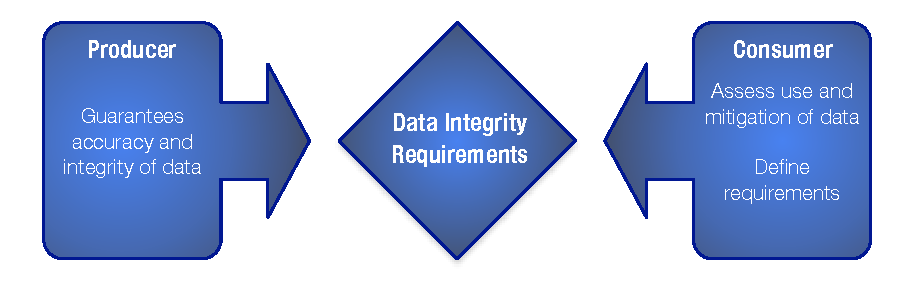
\includegraphics[width=0.75\textwidth]{images/producerconsumer}
  %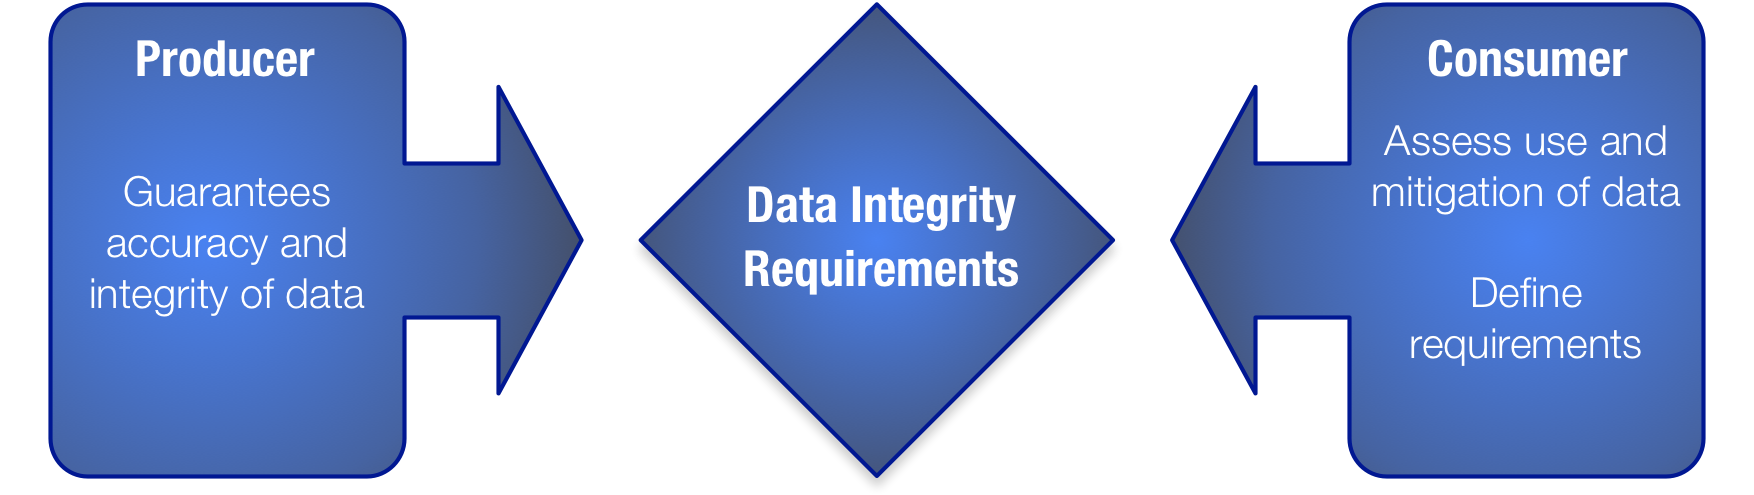
\includegraphics[width=0.75\textwidth]{images/producerconsumer.png}
  \caption{Consumer-focused \index{Integrity Property}\glsfmttext{integrity} requirements}
  \label{fig:producerconsumer}
\end{figure}

The consumer assesses the use of the safety-related data. (In later phases of the data safety management process this \gls{information} is used to define the required \glspl{data property}: for example, how accurate a particular safety-related \index{Artefact, Data}\gls{data artefact} must be.)

The producer investigates how the safety-related data is collected and what errors might occur. (Building on activities in later phases of the data safety management process, the producer can provide some form of guarantee, or level of confidence, that the safety-related data meets the specific data-related requirements.)

In some cases a producer will be providing safety-related data without any knowledge of a specific user (e.g., mapping data or generic \glspl{database} that are sold to many users). In these cases the producer will need to make some assumptions about possible users, and then clearly state what level of \index{Integrity Property}\gls{integrity} the data has been produced to. It is then up to the users to check whether the declared \index{Integrity Property}\gls{integrity} matches their need.

\section{Data in System Lifecycles}
Like other components of a safety-related system, the safety dependency of data is dictated by the context in which it is used and the causal links that become established where loss of one or more of the required \index{Property!Data}properties can contribute to hazardous system states. For example, a given \gls{dataset} (say \gls{configuration data}) could be used in a number of separate contexts such as:
\begin{itemize}
  \item prototyping a system to demonstrate solution feasibility of a safety-related system;
  \item development testing of a safety-related system; and
  \item live operational use of a safety-related system.
\end{itemize}

In these cases, the \gls{dataset} is the same but the context of its use changes the safety significance and therefore the level of assurance that it may require. It follows that the \gls{dsal} of a \gls{dataset} is also predicated on where and when in the lifecycle the \gls{dataset} will be applied. 

To illustrate this concept, a number of generic model lifecycles are discussed below. Note that these are not intended to be prescriptive or mandate the use of any particular model. Instead, they are being used to illustrate how the Data Safety Management Plan could articulate these lifecycle considerations.

\dsiwgTextBF{Development:} the diagram in \autoref{fig:developmentlifecycle} represents a typical development lifecycle using an iterative development approach\footnote{The diagram is based on \gls{ibm}'s Rational Unified Process, an iterative software development\index{Software Development Process} process framework. The original diagram is in the public domain.}. In this model there are key phases as the system transitions from concept through to testable executable code. The process is iterative in that several cycles of functional elaboration, design, development and test may be run and these typically will focus on the areas of the system that bear most technical risk or comprise the key functional use cases so the client gets early visibility of the system. This early awareness allows feedback to be provided into the next iteration to help steer the solution to the client's actual needs. Traditional waterfall implementation can map onto this model on the basis that there is only one iteration in each phase and all activities in one phase need to be completed before progressing to the next.

\begin{figure}[htbp]
  \centering
  %\includegraphics[width=\textwidth]{images/developmentlifecycle}
  %\includegraphics[width=\textwidth]{images/developmentlifecycle_png600}
  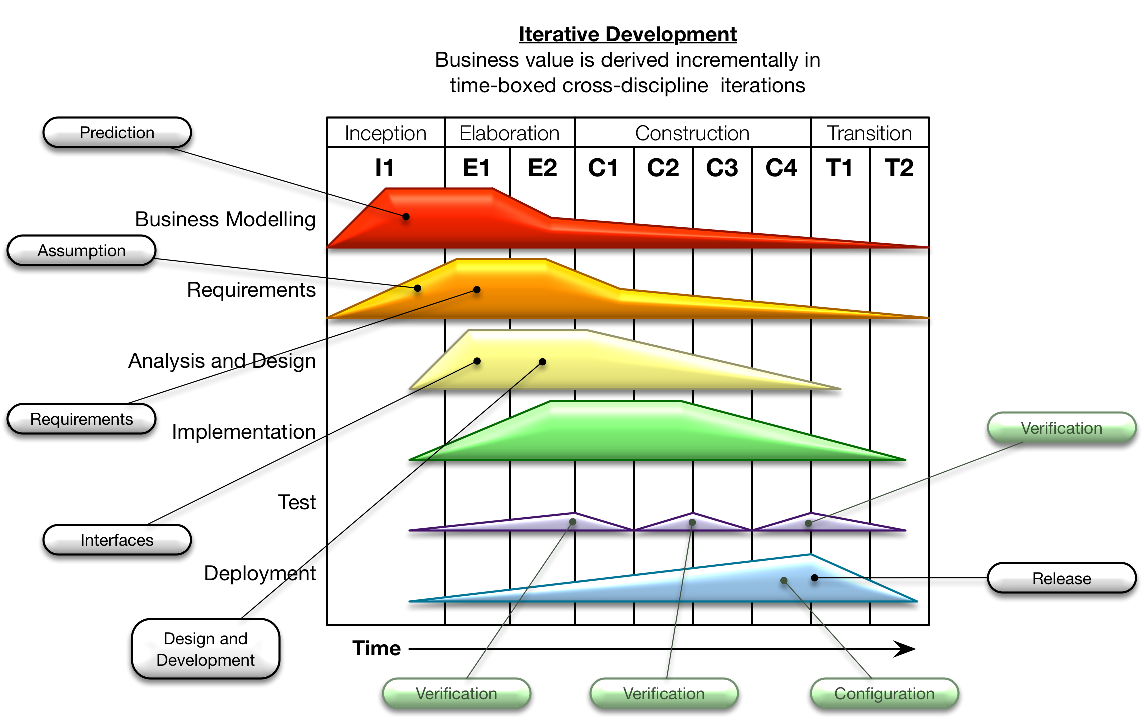
\includegraphics[width=\textwidth]{images/developmentlifecycleflat}
  \caption{Development lifecycle}
  \label{fig:developmentlifecycle}
\end{figure}

The model itself may vary depending on the specific needs of the project but the diagram illustrates that different data categories\index{Category!Data} become significant at different points of the process. 

\dsiwgTextBF{Operational} Once a system has been developed it will move into an operational lifecycle or indeed, if data safety has not previously been considered for an enterprise, then the system could already be in operational use. These operational lifecycles tend to be cyclical in nature; the diagram in \autoref{fig:operationallifecycle}\footnote{ITIL is a registered Trade Mark of AXELOS Limited. All rights reserved.} illustrates a typical model.

\begin{figure}[htbp]
  \centering
  %\includegraphics[width=0.9\textwidth]{images/operationallifecycle}
  %\includegraphics[width=0.9\textwidth]{images/operationallifecycle_png600}
  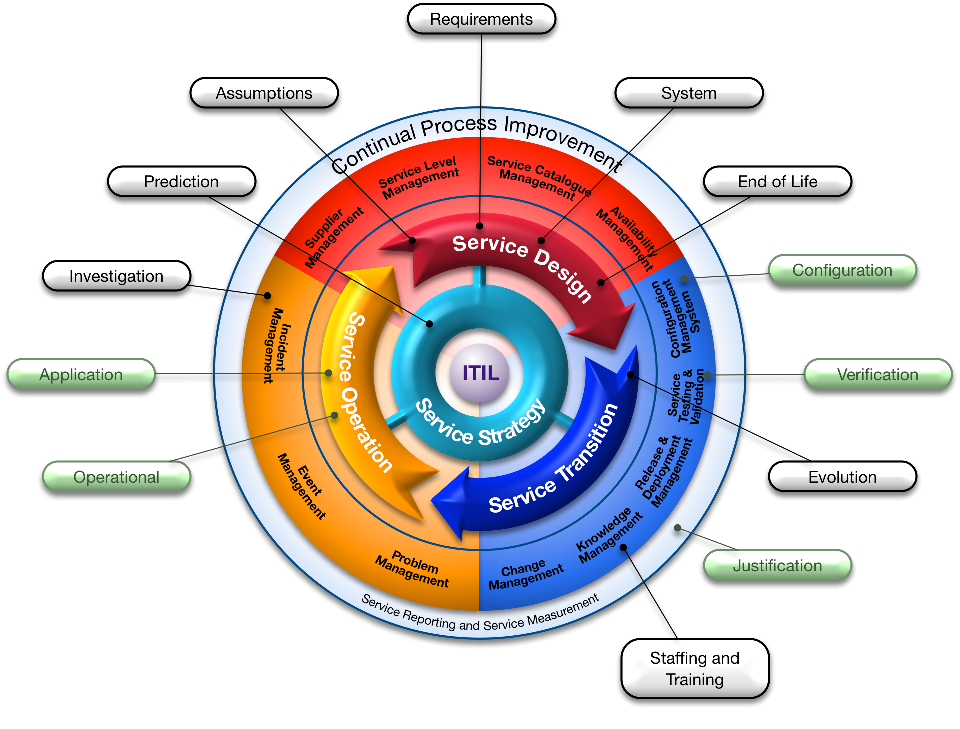
\includegraphics[width=0.9\textwidth]{images/operationallifecycleflat}
  \caption{Operational lifecycle}
  \label{fig:operationallifecycle}
\end{figure}

Again, specific data \index{Category!Data} will come into play at different periods in the process. Documenting the relationship between process steps and data categories will therefore give clarity as to when a particular assurance technique needs to be applied.

\dsiwgTextBF{Data supply chains} The previous models relate to typical system supply and operate perspectives but there are also other data supply chains where a number of organizations engage in the procurement and use of safety-related data. These processes may include the development and operational lifecycles but a different model is required to fully represent the wider processes that are being employed. The diagram in \autoref{fig:dataacquisitionlifecycle} shows such a model representing a data acquisition lifecycle.

\begin{figure}[htbp]
  \centering
  %\includegraphics[width=\textwidth]{images/dataacquisitionlifecycle}
  %\includegraphics[width=\textwidth]{images/dataacquisitionlifecycle_png600}
  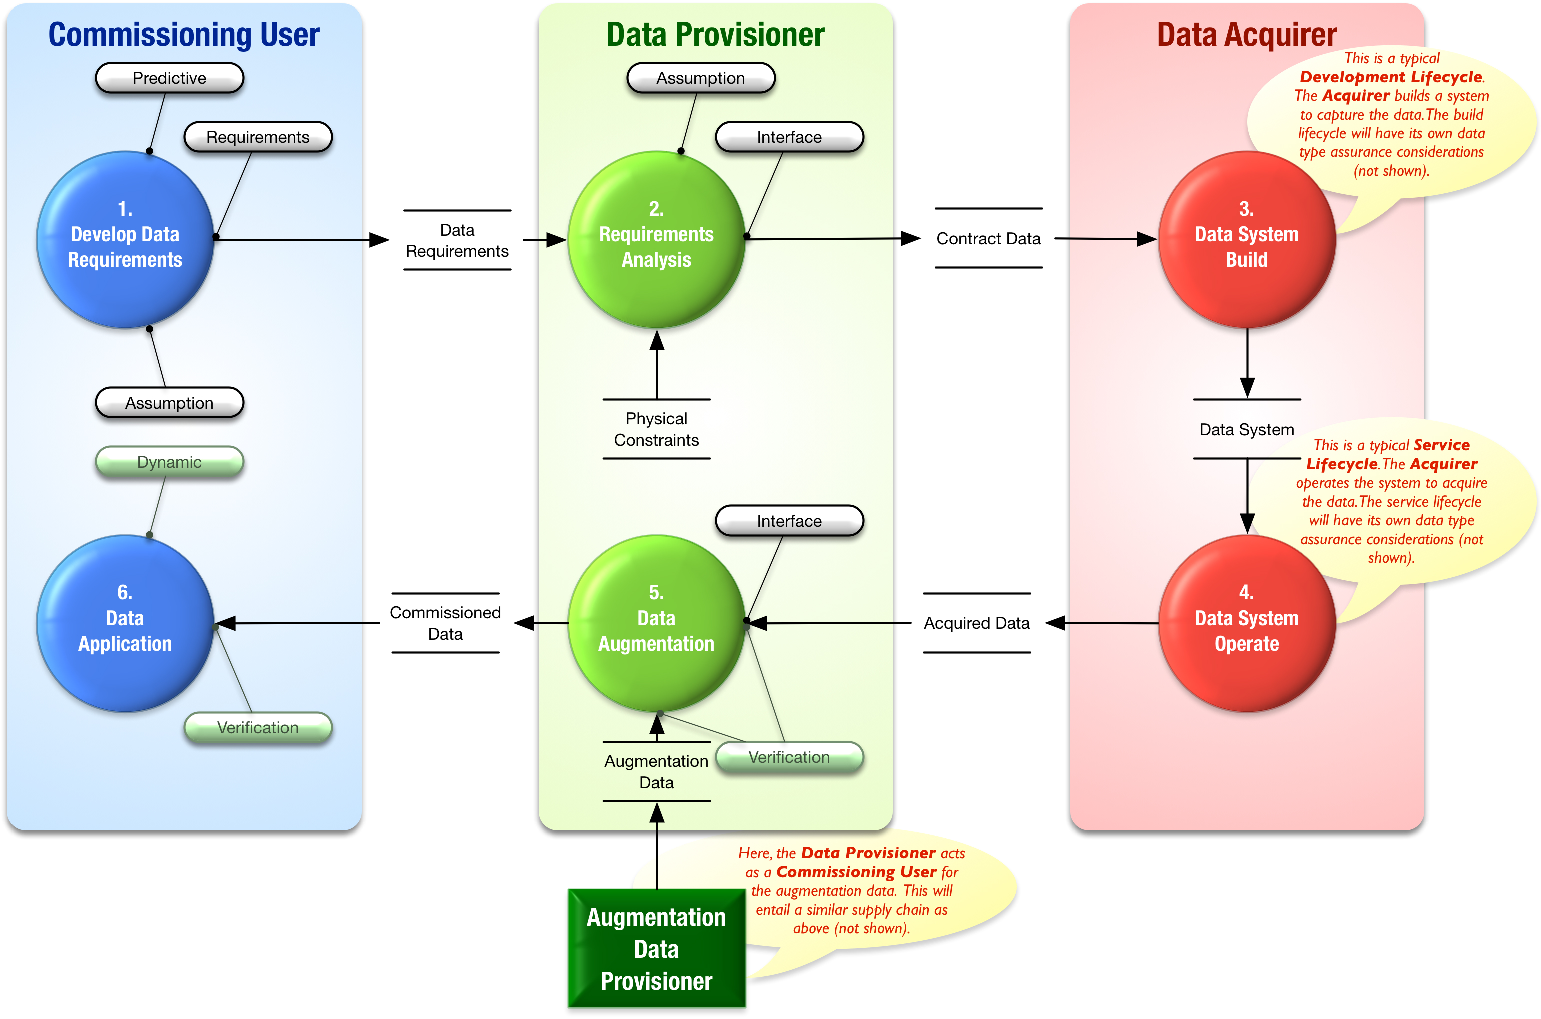
\includegraphics[width=\textwidth]{images/dataacquisitionlifecycleflat}
  \caption{Data supply chain}
  \label{fig:dataacquisitionlifecycle}
\end{figure}

This model represents the interactions between three key organizations:
\begin{itemize}
  \item The commissioning user: the organization that has the need for the data;
  \item The data provisioner: the organization that will fulfil that need for data; and
  \item The data acquirer: the organization employed by the Data Provisioner to carry out physical collection of data.
\end{itemize}

Note that these may be three separate organizations, or they may be separate business units within the same, larger, organization.

In this supply chain, the commissioning user is a consumer of the data and the data acquirer is a producer of data. The data provisioner acts both as a consumer (from the data acquirer) and producer (to the commissioning user) of data. Similarly, an organization that augments \glspl{dataset} is both a consumer and producer of data in the supply chain.

The commissioning user requirement analysis is the key process step where the commissioning user's expectations for data are agreed with the data provisioner. The requirements may be adjusted because of physical constraints (e.g., loss of precision because of physical measuring device constraints) and may include additional requirements to augment the captured data with additional \gls{information} (e.g., airport codes added to a measurement of a given runway length).

The data provisioner may employ a data acquirer to capture the data (e.g., to carry out a physical survey of a site). The acquisition phase may itself require a specialised system to be built to perform the capture and data refinement to meet the data provisioner's specifications. Such systems will then themselves be subject to the development lifecycle model considerations discussed above. Likewise, the data augmentation phase may require further system development processes or indeed, could trigger an instance of the model again as the data provisioner acting as a Commissioning User.

Acquired and augmented data is then fed into the operational system that has been built for providing the service of generating the commissioned data. This system in its service provision role would then typically follow the operational lifecycle process model discussed earlier.

\subsection{Tool Assurance}
Tools in this context are considered anything that automates all or part of a process, for example, data creation or data transformation. Test tools are also included (i.e., the term is not limited to parts of an operational system).

Tools can impact data safety in different ways, depending on both their function and how they are to be used. For tools to be considered fit for purpose it is necessary to show that the tool meets its requirements in the context in which it is to be used. The activity to ensure a tool is fit for purpose is usually called ``tool qualification''.

The first step is to define the purpose for which the tool is required to be fit. Once that is done, and the tool's requirements are specified, there are three main strategies available for qualification:
\begin{itemize}
  \item Use evidence of a previous certification of the tool by a trusted third party (unlikely to be available in most industry sectors);
  \item Base tool qualification on the practices used when designing and developing the tool (only practicable for tools developed within the organization); and
  \item Use one of the available industry-specific guidance documents that admit \gls{cots} solutions, e.g., EUROCAE Document ED-215 (RTCA/DO-330) \cite{citation:ED215}.
\end{itemize}

%There is an alternative, risk-based and perhaps more feasible, approach. This involves assessing the potential risks presented by use of the tool and providing assurance that these risks are adequately managed. The method proceeds as follows:

%\begin{itemize}
%  \item Draft a procedure for the use of the tool to achieve the stated purpose;
%  \item Identify threats to data safety associated with using the tool;
%  \item Specify adequate mitigations\index{Mitigation} for each identified threat;
%  \item Augment and formally issue the tool requirements and the usage procedure to implement the specified  mitigations\index{Mitigation%};
%  \item Demonstrate that the tool and its mitigations\index{Mitigation} perform as expected; and
%  \item Provide a compelling assurance argument based on the previous steps and any other evidence that will improve confidence; for example:
%  \begin{itemize}
%    \item reputation of the supplier; 
%    \item configuration management of the tool, its settings and its documentation;
%    \item competence of the tool user; and
%    \item checks that are made on the tool's output.
%   \end{itemize}
%\end{itemize}

Further details on tool qualification are presented in \dsiwgRef{Appendix}{bkm:tools}.

\subsection{Test Data}
The generation of suitable test data is critical to verification of a safety system. The test data must include both representative ``normal'' values based on intended usage and also values which push at, and beyond, normal use to provoke \glspl{hazard} that the system might produce. This latter type of test data is particularly hard to generate; generally it must be credible, yet it must stress the system to react in a way that the preservation of \index{Property!Safety}safety properties can be assessed. 

In general, all the \index{Property!Data}properties of the test data should be considered and an assessment made as to whether breaking a property (e.g., introducing corrupt or late data) would cause a problem to the system. If it does, then specific test data should be produced to facilitate testing of this potential problem.

Some suggestions for test data for safety-related systems are:
\begin{itemize}
  \item Use of values on or around boundaries;
  \item Use of extreme values, way beyond what could be reasonably expected;
  \item Use of typical ``everyday'' values / sets;
  \item Some realistic but unexpected values;
  \item Try combinations of data values or \glspl{item data} that are problematic together (e.g., inconsistent);
  \item If possible, use some values known to have caused problems in the past;
  \item Where appropriate, use values related to timing, rollover or date boundaries;
  \item Where possible, use white box values (i.e., those derived from an understanding of the system);
  \item Use a set of values with drift or bias over time;
  \item Use \glspl{dataset} with particular \index{Property!Statistical}statistical properties (e.g., distribution, patterns etc.);
  \item Use data which has incorrect formatting, ordering, or out of sequence, etc.; and
  \item Try data which has repeated sets of values or pseudo-random characteristics.
\end{itemize}
Typically very complex test data is derived from recorded live feeds of real data flows. While this data can be extremely useful for regression purposes, it should be recognised that it is unlikely to contain many outlying or boundary \glspl{item data}. Therefore it may need to be modified to test any hazardous situations; this modification can be difficult and may require sophisticated tools to both ensure correct \index{Property!Data}properties and injection of the intended faults (for instance to introduce a statistical bias to the data).

Simulator / emulator derived values can be useful, but again the issue is how realistic the values are: often the \index{Accuracy Property}\gls{accuracy}, \gls{resolution} or timing of simulated values may be different to real data.

Coverage with test data is something to consider. Sometimes the same \gls{dataset} is used for multiple test scenarios, when in fact it is not stressing all of them to the same degree. Test data coverage can be collected over requirements, code or design, but it is important not to forget hazards: coverage of the hazards and mitigations\index{Mitigation} identified in the \gls{hazard log} is a key aim. 

In general some measure of the quality and suitability of the test data can be useful. This could be based on \index{Property!Statistical}statistical properties, coverage of hazards or coverage of requirements. 

Test data must show continued relevance, through systems evolution\index{Evolution!System} and over time. It is good practice to build up extensive regression suites containing coverage of all detected problems to date.

\subsection{Interfaces with Existing Assessments}\index{Interface!Assessment}
\subsubsection{Data and Software}\index{Software vs. Data}
Although most people feel they have an intuitive understanding of the difference between software and data, upon closer examination the boundary is not always as clear as it may first appear.

Consider, for example, Java bytecode, which is operated on by a Java virtual machine. From one perspective, it could be argued that the Java bytecode is simply data. By extension, it could also be argued that the Java source code is also just data. This type of argument can be extended to suggest that any software\index{Software vs. Data} can, at least from one viewpoint, be considered as data. Conversely, think about the data used in a 3D printer, perhaps to produce a part for an aircraft. This data could be viewed as a program for the printer; that is, it could potentially be viewed as software. This type of argument can easily be extended across a range of situations, especially those relating to \gls{configuration data}.

While they are interesting, and potentially important, these philosophical considerations should not detract from the practical issue: there are some aspects of data (using the term in a generic sense) that are often not explicitly addressed in standards. These are a consequence of features that are more readily apparent in data than in software\index{Software vs. Data}. Examples include:
\begin{itemize}
  \item It is easy for data to be reused in a range of contexts and despite appearances it is not trivial to translate an assurance argument that the data is fit for purpose from one context to another.
  \item It is not always clear who owns or is responsible for data, especially when data is shared and processed amongst a collection of disparate systems.
	\item Data often has a \gls{lifetime}, that is a time after which it is no longer valid. This may be a strict cut off, or a more gradual degradation in the utility (or applicability) of the data.
  \item There is often a default value for data. While this can make systems easier to use and hence more productive it can be difficult to identify a default value that is appropriate for all circumstances.
  \item It can be easy to change data. In some circumstances this can give rise to a temptation to make uncontrolled and potentially untested changes. It can also allow data to be fraudulently changed after an accident.
\end{itemize}
In summary, data and software\index{Software vs. Data} are closely related and, as such, need to be considered together in system engineering activities, including system safety analyses. However, data and software emphasise different facets of risk and they are susceptible to different mitigation\index{Mitigation} approaches; this means there is also a need to adopt a data-focused perspective. It also means that \index{Assurance Level!Software}\glspl{software assurance level} cannot be mapped directly to \index{Assurance Level!Data}\glspl{dsal}.

\subsubsection{Data Safety and Security}
When generating high-level processes and techniques to manage the risks posed by data, it is worthwhile understanding the difference between the safety risks posed by accidental failure to preserve \index{Property!Data}Data Properties and the security risks posed by actors maliciously undermining the properties of data.

The relationship between safety and security, as engineering concepts, can be summarised by their relationships to cultural, developmental and aspirational \index{Property!System Development}properties of systems development.

Culturally, embedding both safety and security into an organization is seen as a key strategic goal for creating systems that are both safe and secure. Developmentally, safety and security are quality factors, generating transverse requirements that impact the entire system. Most importantly, at the aspirational level, both safety and security have the common goal of preventing harm from accidental and malicious interventions respectively.

For an organization aiming to create systems that are both safe and secure, these connections can be both a benefit and a burden. The shared goal of preventing harm means that both quality factors seek to identify routes to harm through analysis of the system being developed. This can result in shared processes and tools, which in turn can save time and money during systems development. However, safety and security interact in a more volatile way at the functional level. Security failings can undermine the safety case for a system and, conversely, \index{Safety Requirement}safety requirements can prevent the implementation of standard security solutions. For example, the German government published a report in 2014 into a fire at a steel works caused by a cyber attack that resulted in the control system being placed into an unsafe state and the safety system being unable to intervene (Section 3.3.1 of \cite{citation:DieLage} - in German). In addition, ``fail-safe'' states can often leave a system with exposed security vulnerabilities.

These links between safety and security infer that there are connections between the sub-categories of data safety and \gls{information} security: both attempt to take a data-centric view of the system of interest in order to improve the associated quality factor; and both attempt to prevent harm through the preservation of the \index{Property!Data}properties of data within that system.

In the security domain, the three key properties of data considered are \gls{confidentiality}, \index{Integrity Property}\gls{integrity}, and \gls{availability}. \Gls{confidentiality}, the failure of which is termed ``\gls{information} disclosure'' in the Microsoft Security Model, \cite{citation:leblanc2002writing} is typically not a safety concern as, without malicious intent, \gls{information} sharing is not inherently unsafe. However, when considering systems where \gls{confidentiality} is an important property, the interaction between data safety and security cannot be trivially resolved. For example, accidental disclosure of \gls{information} can form part of a causal chain which leads to harm from a malicious actor.

Data \index{Integrity Property}\gls{integrity} is a critical property for both domains. The Microsoft Security Model describes malicious removal of the property of \index{Integrity Property}\gls{integrity} as ``tampering''. Whether by accident or through malicious intent, the potential harm from loss of data \index{Integrity Property}\gls{integrity} can be disastrous to a safety-critical system, from the values of drug dosages to control system parameters. 

Data \gls{availability} is also important to both domains. Loss of \gls{availability}, or ``denial of service'' in the Microsoft Security Model, is another \index{Property!Data}property that can be lost accidentally or through malicious intervention. Loss of \gls{availability} prevents systems from functioning properly and can result in undefined behaviour if not mitigated\index{Mitigation} by design.

Further guidance on the integration of safety and security can be found in a code of practice published by the IET
\cite{citation:IetCyber}.
The Code of Practice is written for engineers and engineering management to support their understanding of the issues
involved in ensuring that the safety responsibilities of an organization are addressed, in the presence of a threat of
cyber attack.

%================================================================================
%       Safety Critical Systems Club - Data Safety Initiative Working Group
%================================================================================
%                       DDDD    SSSS  IIIII  W   W   GGGG
%                       D   D  S        I    W   W  G   
%                       D   D   SSS     I    W W W  G  GG
%                       D   D      S    I    WW WW  G   G
%                       DDDD   SSSS   IIIII  W   W   GGG
%================================================================================
%               Data Safety Guidance Document - LaTeX Source File
%================================================================================
%
% Description:
%   Appendix addressing data migration
%================================================================================
\chapter{Data Migrating, Porting, Importing and Exporting (Informative)}\index{Data Migration}\label{bkm:migration}
%
%\dsiwgSectionQuote{The whole story of migration and what that has done in interconnecting the planet is obviously something I've written about a lot}{Salman Rushdie}
%\dsiwgSectionQuote{Migration is an expression of the human aspiration for dignity, safety and a better future. It is part of the social fabric, part of our very make-up as a human family}{Ban Ki-moon}
%\dsiwgSectionQuote{When it's well managed, migration works in the national interest, for our communities, economy and country.}{Priti Patel}
%\dsiwgSectionQuote{I think migration is a right, but it should be an option, not an obligation}{Nayib Bukele}
\dsiwgSectionQuote{I don't think you'll ever have a perfect world because we humans are prone to error, and so we're always in search of an upgrade}{Henry Rollins}

Migrating, Porting and Import or Export of data between systems is a large and complex topic.
This appendix highlights some of the issues that arise, links to the data safety properties and suggests some mitigations.

\section{Introduction and rationale}\label{bkm:migrationintro}
All of these activities involve moving data around, with the expectation that the data will be re-used or re-purposed to some extent after the move. Why is this a problem? Because data can be lost, transformed or misinterpreted due to the migration. If some of this data is safety-related then there is the possibility of creating a data \gls{hazard}. The worst cases are the silent ones: where data is not migrated or modified or changed into something else on migration, and no notification or warning is provided.
In general porting of data, import and export actions can be considered subsets of full data migration activities. 
The following are typical stages of a data migration exercise:
\begin{enumerate}[label=\color{dsiwgAccentColour}\roman*)]
\item Discovery: Identifying what data has to be migrated:
the history, locations, store types, formats and the software currently used to manipulate it.
\item Analysis and Preparation:
Filtering and sorting the data, identifying and cleansing the data, fixing any issues, creating missing data that can’t be moved,
and transforming the data to make it suitable for use in the new system.
\item Trials:
Selected sets or portions of the data are migrated and the results assessed within the new system or context.
This may be extended to include more data through incremental, phased stages.
\item Dry Run:
A full migration is performed to a duplicate system or to the new system in a way that it can be backed out
(ie. the new system can be reverted to its original state), and use of the current system can be continued if necessary.
\item Parallel Running:
Both old and new systems continue running, processing the same data where possible.
This is desirable as it allows quick reversion to the old system in case of failure.
It also allows (sampling) comparison between the old and new systems outputs.
\item Monitoring and Checking:
Operation of the new system is closely monitored and outputs assessed to establish if these would be similar to those produced
by the old system.
\item Move to New:
This is where the old system is switched off and mothballed, and may be subsequently decommissioned and removed.
\end{enumerate}

It is noted that migration is generally between systems
(e.g. a legacy system and a new one) but can be between different instances or environments within the same system,
involving different software, stores or \glspl{database}.

Many moves of data are now to Cloud storage, and the implementation may be largely hidden,
with only software API interfaces available\footnote{It is noted that within a cloud environment mini automated migrations of data are happening all the time as new servers and storage are provisioned by the service provider, software is upgraded, etc. There should be some sort of assurance provided in this case to ensure the data is preserved as required.}.
In this case the options for comparisons may be more limited.
%
\section{Migration Cases}
%
There are at least three cases of migration (these simple diagrams are intended to show the end state of the migration, it is acknowledged that there are intermediate stages, as mentioned in \dsiwgRef{Section}{bkm:migrationintro}):
\begin{enumerate}
\item Migration of data from a single old system to a single new system.
This is very common and is the usual upgrade path.
The new system, or indeed both systems, may be in the Cloud.

\begin{figure}[htbp]
  \centering
  
\includegraphics[width=\textwidth/2]{images/migration1.pdf}
  \caption{Simple migration path\index{Data Migration!Simple}}
  \label{fig:migration1}
\end{figure}

\item Migration of data from multiple disparate systems to one new system.
This is less common but can be seen in major technology upgrades where it is seen as beneficial to bring together multiple
legacy systems into one new system.

\begin{figure}[htbp]
  \centering
  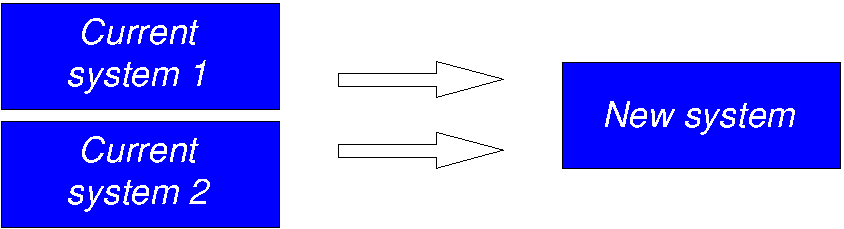
\includegraphics[width=\textwidth/2]{images/migration2.pdf}
  \caption{Many-to-one migration path\index{Data Migration!Many to one}}
  \label{fig:migration2}
\end{figure}

\item Migrating data back to an old system in case of failures or to investigate data issues with the new system

\begin{figure}[htbp]
  \centering
  
\includegraphics[width=\textwidth/2]{images/migration3.pdf}
  \caption{Reversion migration path\index{Data Migration!Reversion}}
  \label{fig:migration3}
\end{figure}

\end{enumerate}
%
\section{Safety issues due to migration}
%
The following table summarises some of the safety issues due to migration, maps these to the data safety properties and gives possible mitigations.

\begin{longtable}{|C{\dsiwgColumnWidth{0.10}}|C{\dsiwgColumnWidth{0.24}}|C{\dsiwgColumnWidth{0.20}}|C{\dsiwgColumnWidth{0.20}}|C{\dsiwgColumnWidth{0.20}}|}
  \caption{Safety issues due to migration}
  \label{tab:migration}
  \\\hline
  \TableHeadColourCX{No.} & \TableHeadColourCX{Migration Case} & \TableHeadColourCX{What are safety issues in each case?} & \TableHeadColourCX{Mapping to properties/loss of properties} & \TableHeadColourCX{Possible Mitigations (Table \ref{tab:MethodsDataMigration})}\\\hline
  \endfirsthead
  \caption[]{Safety Issues due to Migration (continued)}
  \\\hline
  \TableHeadColourCX{No.} & \TableHeadColourCX{Migration Case} & \TableHeadColourCX{What are safety issues in each case?} & \TableHeadColourCX{Mapping to properties/loss of properties} & \TableHeadColourCX{Possible Mitigations (Table \ref{tab:MethodsDataMigration})}\\\hline
  \endhead
  \multicolumn{5}{r}{\sl Continued on next page}
  \endfoot
  \endlastfoot

1.&
Data format may not map exactly: due to different \gls{database} formats, word lengths, endian issues, etc.&
Data can be lost or discarded, or substituted for defaults. Data may be migrated / imported / exported incorrectly.&
\Gls{integrity}, \gls{completeness}, \gls{format}&
DM.02, DM.07, DM.08, DM.09, DM.10\\\hline
%
2.&
Data may not translate exactly: no equivalent data type / record / field type in new system, etc&
Data can be lost or discarded, or substituted for defaults. Data may be migrated / imported / exported incorrectly.&
\Gls{integrity}, \gls{completeness}&
DM.02, DM.04, DM.07, DM.08, DM.09, DM.10\\\hline
%
3.&
Data may not be valid: less numeric range available in new system, etc. Subtype of (2).&
Data can be lost or discarded, or substituted for defaults. Data may be migrated / imported / exported incorrectly.&
\Gls{integrity}, \gls{completeness}&
DM.02, DM.04, DM.07, DM.08, DM.09, DM.10\\\hline
%
4.&
\Gls{metadata} (data about the data) may be lost, including \gls{data dictionary} aspects, derivation, history, signoffs, authorisations,
logs, etc.&
Data may be migrated / imported / exported losing \gls{information}.&
\Gls{traceability}, \gls{history}\index{History Property}&
DM.04, DM.09\\\hline
%
5.&
Data may have a different meaning or interpretation in the new system context.
E.g. if a fluid value is ‘gallons’ and this is migrated from a UK to a US-developed system without applying an adjustment factor.&
Meaning of data can be altered even if migration apparently successful.&
\Gls{consistency}, \gls{fidelity}&
DM.01, DM.04, DM.11\\\hline
%
6.
&
Data may be correctly rejected (detection of error on import / export)&
Data is lost. Not necessarily a problem if notified and fixed.&
\Gls{completeness}&
DM.07, DM.08, DM.09, DM.10\\\hline
%
7.
&
Data may be wrongly filtered or rejected as incompatible&
Correct data is rejected. If data can’t be imported what should happen? a. Rejected and migration halted,
b. Rejected and notified, c. Rejected silently, d. Substituted?&
\Gls{integrity}, \gls{completeness}&
DM.02, DM.03, DM.07, DM.08, DM.09, DM.10\\\hline
%
8.&
Two or more \glspl{item data} may map to the same item in the new system – one may overwrite the other with the last one ‘winning’.&
This is a case of aliasing (See 6.2.2 ref). Data can be lost or discarded. Data may be migrated / imported / exported incorrectly.&
\Gls{integrity}, \gls{completeness}&
DM.02, DM.03, DM.07, DM.08, DM.09, DM.10\\\hline
%
9.&
There may be situations where the data store has to be ‘live’ and the migration / import / export process takes some time.
In this case some data may be out of date and become inconsistent (stale), and \gls{integrity} of the whole \gls{dataset} is lost.&
Data may be migrated / imported / exported incorrectly.&
\Gls{consistency}, \gls{integrity}, \gls{timeliness}&
DM.07, DM.08\\\hline
%
10.&
If a migration is unsuccessful, data changes may have to be undone and stores reverted to original state.
This may not always be possible or completely done.&
Original \gls{dataset} may be corrupted.&
\Gls{consistency}, \Gls{integrity}&
DM.06, DM.07, DM.08\\\hline
%
11.&
The data ‘cleansing’ activity conducted before or during migration may introduce faults.&
The cleansing activity may miss some data faults or may be over-zealous, deleting good values.&
\Gls{integrity}, \gls{completeness}&
DM.07, DM.09, DM.13\\\hline
\end{longtable}

%================================================================================
%       Safety Critical Systems Club - Data Safety Initiative Working Group
%================================================================================
%                       DDDD    SSSS  IIIII  W   W   GGGG
%                       D   D  S        I    W   W  G   
%                       D   D   SSS     I    W W W  G  GG
%                       D   D      S    I    WW WW  G   G
%                       DDDD   SSSS   IIIII  W   W   GGG
%================================================================================
%               Data Safety Guidance Document - LaTeX Source File
%================================================================================
%
% Description:
%   Proposed alternate ways to customise the assignment of DSALs 
%
%================================================================================
\chapter{\glsfmtshort{dsal}\index{Assurance Level!Data} Customisation (Informative)} \label{bkm:DsalCustomisation}
%\dsiwgSectionQuote{Common sense tells us that the government's attempts to solve large problems more often create new ones. Common sense also tells us that a top-down, one-size-fits-all plan will not improve the workings of a nationwide health-care system that accounts for one-sixth of our economy}{ Sarah Palin}

\dsiwgSectionQuote{One size does not fit all}{Frank Zappa}

%\dsiwgSectionQuote{When we make decisions in our personal and professional lives, we typically start with some form of data. The very word ‘data’ derives from the Latin meaning ‘something given’. But who gave it? Where is it from? Should I accept it at face value?}{Adrian Smith CEO of the Alan Turing Institute}
\section{Introduction}
Within the body of this document, a method has been provided for the assignment of \glspl{dsal}\index{Assurance Level!Data}. However it is anticipated that, as with the methods used for the assignment of safety criteria within system safety analysis, some programmes may find it desirable to develop alternate approaches. This section presents some possible methods for the determination of likelihood. These methods are intended to serve as approaches for consideration when developing project-specific criteria, as these approaches are less generic than that presented through \autoref {tab:Likelihood}, so it is highly likely that customisation will be required.

\section{Significance factors}
\label{bkm:SignificanceFactors}
A method of determining likelihood from the different characteristics is to implement a scoring scheme that apportions a quantitative value for each of the characteristics, with the sum giving the total likelihood score. The total score is then compared against a scale, and that in turn determines the overall low, medium or high assessment.

For example, consider the modified version of \autoref {tab:Likelihood} illustrated in \autoref {tab:Likelihood1}

\begin{longtable}{|C{\dsiwgColumnWidth{0.19}}|C{\dsiwgColumnWidth{0.27}}|C{\dsiwgColumnWidth{0.27}}|C{\dsiwgColumnWidth{0.27}}|}
  \caption{Calculation of likelihood -- option 1}
  \label{tab:Likelihood1}
  \\\hline
  \TableHeadColour{} & \multicolumn{3}{c|}{\TableHeadColourCX{Score}}\\\cline{2-4}
  \multirow{-2}*{\TableHeadColourCX{}} & \TableHeadColourCX{2} & \TableHeadColourCX{1} & \TableHeadColourCX{0}\\\hline
  \endfirsthead
  \caption[]{Calculation of likelihood -- option 1 (continued)}
  \\\hline\TableHeadColour{} & \multicolumn{3}{c|}{\TableHeadColourCX{Score}}\\\cline{2-4}
  \multirow{-2}*{\TableHeadColourCX{}} & \TableHeadColourCX{2} & \TableHeadColourCX{1} & \TableHeadColourCX{0}\\\hline
  \endhead
  \multicolumn{4}{r}{\sl Continued on next page}
  \endfoot
  \endlastfoot
  Proximity & %
    A known use of the data is highly likely to lead to an accident. & %
    A possible use of the data could lead to an accident. & %
    All currently foreseen uses of the data could lead to harm only via lengthy and indirect routes.\\
    \hline
  Dependency & %
    Data is completely relied upon. & %
    Data is indirectly relied upon. & %
    Little reliance on data.\\
    \hline
  Prevention & %
    Difficult or impossible to guard / barrier against errors. & %
    Possible to guard / barrier against errors. & %
    Easy to guard / barrier against error.\\
    \hline
  Detection & %
    Low or no chance of anything else detecting an error. & %
    Some other people / systems are involved in checking the data. & %
    Many other people / systems are involved in checking the data.\\
    \hline
  Correction & %
    Difficult or impossible to correct or workaround errors. & %
    Possible to correct or workaround errors. & %
    Easy to correct or workaround errors.\\
    \hline
\end{longtable}

For each of the characteristics, the applicable assessment of likelihood is then selected and scored. So for example, if it is “Possible to guard / barrier against errors” for Prevention, then the score for that characteristic would be 1. Each characteristic is then scored and they are then summed to give a total score. The range of possible values will run from 0 (all choices in the far right column, favouring low likelihood aspects) through to 10 (all choices in the far left column, favouring high likelihood aspects).

The overall likelihood in the assessed against a scale such that shown in \autoref{tab:Likelihood1a}.

\begin{longtable}{|C{\dsiwgColumnWidth{0.2}}|C{\dsiwgColumnWidth{0.2}}|C{\dsiwgColumnWidth{0.2}}|}
  \caption{Likelihood assessment}
  \label{tab:Likelihood1a}
  \\\hline
%  \TableHeadColour{} & \multicolumn{3}{c|}{\TableHeadColourCX{Likelihood}}\\\cline{2-4}
  \TableHeadColourCX{Low} & \TableHeadColourCX{Medium} & \TableHeadColourCX{High}\\\hline
  \endfirsthead
  \caption[]{Likelihood assessment (continued)}
  \\\hline
%  \TableHeadColour{} & \multicolumn{3}{c|}{\TableHeadColourCX{Likelihood}}\\\cline{2-4}
  \TableHeadColourCX{Low} & \TableHeadColourCX{Medium} & \TableHeadColourCX{High}\\\hline
  \endhead
  \multicolumn{3}{r}{\sl Continued on next page}
  \endfoot
  \endlastfoot
  0--2 & 3--6 & >6\\\hline
\end{longtable}


\section{Weighted characteristics}
The method presented in
\dsiwgRef{section}{bkm:SignificanceFactors}
may be enhanced to provide a more holistic overall assessment of the likelihood based on all characteristics. Note that the scheme in
\dsiwgRef{section}{bkm:SignificanceFactors}
allocated equal significance to each of the characteristics. This method could be further refined if necessary to apply weightings to each of the characteristics, as shown in \autoref{tab:Likelihood2}.

\begin{longtable}{|C{\dsiwgColumnWidth{0.19}}|C{\dsiwgColumnWidth{0.15}}|C{\dsiwgColumnWidth{0.20}}|C{\dsiwgColumnWidth{0.20}}|C{\dsiwgColumnWidth{0.20}}|}
  \caption{Calculation of likelihood -- option 2}
  \label{tab:Likelihood2}
  \\\hline
  \TableHeadColour{} & \TableHeadColour{} & \multicolumn{3}{c|}{\TableHeadColourCX{Score}}\\\cline{2-4}
  \multirow{-2}*{\TableHeadColourCX{}} & \TableHeadColourCX{Weighting} & \TableHeadColourCX{2} & \TableHeadColourCX{1} & \TableHeadColourCX{0}\\\hline
  \endfirsthead
  \caption[]{Calculation of Likelihood -- Option 2 (continued)}
  \\\hline
  \TableHeadColour{} & \TableHeadColour{} & \multicolumn{3}{c|}{\TableHeadColourCX{Score}}\\\cline{2-4}
  \multirow{-2}*{\TableHeadColourCX{}} & \TableHeadColourCX{Weighting} & \TableHeadColourCX{2} & \TableHeadColourCX{1} & \TableHeadColourCX{0}\\\hline
  \endhead
  \multicolumn{4}{r}{\sl Continued on next page}
  \endfoot
  \endlastfoot
  Proximity & %
    1.5 & %
    \bf A known use of the data is highly likely to lead to an accident. & %
    A possible use of the data could lead to an accident. & %
    All currently foreseen uses of the data could lead to harm only via lengthy and indirect routes.\\
    \hline
  Dependency & %
    1.0 & %
    Data is completely relied upon. & %
    \bf Data is indirectly relied upon. & %
    Little reliance on data.\\
    \hline
  Prevention & %
    1.3 & %
    \bf Difficult or impossible to guard / barrier against errors. & %
    Possible to guard / barrier against errors. & %
    Easy to guard / barrier against error.\\
    \hline
  Detection & %
    0.7 & %
    Low or no chance of anything else detecting an error. & %
    Some other people / systems are involved in checking the data. & %
    \bf Many other people / systems are involved in checking the data.\\
    \hline
  Correction & %
    0.5 & %
    Difficult or impossible to correct or workaround errors. & %
    Possible to correct or workaround errors. & %
    \bf Easy to correct or workaround errors.\\
    \hline
\end{longtable}

The total score is then calculated by first multiplying the individual characteristic’s score by the weighting before summing all the values. For example, if the selections highlighted in bold were made, then the score would be
$$(1.5 \times 2) + (1.0 \times 1) + (1.3 \times 2) + (0.7 \times 0) + (0.5 \times 0) = 6.6$$
resulting in a {\sl High} assessment rather than the {\sl Medium} that would result with no weighting. This is because Proximity and Prevention are considered (in this particular example) more important than Detection and Correction. The weightings within a project-specific version of this table would be chosen by the organization to suit the particular scenario under consideration.

\backmatter
\include{Acronyms}
\include{References}
%================================================================================
%       Safety Critical Systems Club - Data Safety Initiative Working Group
%================================================================================
%                       DDDD    SSSS  IIIII  W   W   GGGG
%                       D   D  S        I    W   W  G   
%                       D   D   SSS     I    W W W  G  GG
%                       D   D      S    I    WW WW  G   G
%                       DDDD   SSSS   IIIII  W   W   GGG
%================================================================================
%               Data Safety Guidance Document - LaTeX Source File
%================================================================================
%
% Description:
%   Acknowledgements section.
%
%================================================================================
\section{Acknowledgements (Discursive)} \label{bkm:acknowledgements}

\dsiwgSectionQuote{Our ability to do great things with data will make a real difference in every aspect of our lives.}{Jennifer Pahlka}

The document contributors would like to thank:
\begin{itemize}
  \item The \gls{scsc}.
  \item The \gls{scsc} Covid-19 Working Group for providing some of the data used in the Covid-19 Appendix.
  \item Brian Jepson of the \gls{scsc} for web hosting support and technical help with the \gls{scsc} web site.
  \item
    Tim Rowe for editing this edition.
  \item Paul Hampton
    and
    Mark Templeton for managing the publication processes.
  \item
    Nick Hales, Mike Parsons, Tim Rowe, Alan Simpson and Mark Templeton
    for developing the additional text for this edition.
  \item
    Martin Atkins and Divya Atkins for driving the development of tooling and promoting data safety.
  \item Mike Parsons for chairing the Working Group meetings.
  \item All those who have taken minutes at Working Group meetings.
  \item
    All the organisations that have hosted Working Group meetings.
  \item All the organisations that have provided support to the document's contributors.
  \item Those that have been unable to attend meetings but have made supporting contributions.
\end{itemize}

%================================================================================
%       Safety Critical Systems Club - Data Safety Initiative Working Group
%================================================================================
%                       DDDD    SSSS  IIIII  W   W   GGGG
%                       D   D  S        I    W   W  G   
%                       D   D   SSS     I    W W W  G  GG
%                       D   D      S    I    WW WW  G   G
%                       DDDD   SSSS   IIIII  W   W   GGG
%================================================================================
%               Data Safety Guidance Document - LaTeX Source File
%================================================================================
%
% Description:
%   Contributors section.
%
%================================================================================
\chapter{Contributors (Discursive)} \label{bkm:contributors}

\dsiwgSectionQuote{Without data, you're just another person with an opinion.}{W. Edwards Deming}

This document has had the benefit of contributions from a large number of people, who work for a variety of organisations, which collectively span a range of different sectors. Note that contributions  have been made on an individual basis and, in particular, the inclusion of an organisation in the following list does \dsiwgTextBF{not} necessarily mean that organisation agrees with the entire contents of the document.

Updates to the most recent version of the document were written by:
\begin{itemize}
  \item Divya Atkins, Mission Critical Applications
  \item Martin Atkins, Mission Critical Applications
  \item Paul Hampton, CGI IT UK Ltd
  \item Mike Parsons, Ebeni and \gls{scsc}
  \item Tim Rowe, TGR Safety Management Ltd
\end{itemize}

%Review comments were gratefully received from the following:
%\begin{itemize}
%\item Oscar Slotosch, Validas AG
%\item Andy Williams
%\end{itemize}
  
%\clearpage %Manual page break
In addition to the above,
contributors to earlier versions upon which this document is based include the following
(the organisations listed were correct at the time of their contribution)
:
\begin{itemize}
  \item Mike Ainsworth, Ricardo
  \item Rob Ashmore, Dstl
  \item Michael Aspaturian, EDF Energy
  \item Janette Baldwin, Thales UK
  \item Dave Banham, Blackberry QNX
  \item Ian Bingham
  \item John Bragg, MBDA UK Ltd
  \item Jennifer Brain, Wood plc
  \item Eric Bridgstock
  \item Simon Brown, QinetiQ
  \item Dermot Martin Burke, BAE Systems
  \item Dale Callicott, DKCSC Ltd
  \item John Carter, General Dynamics
  \item Martyn Clarke, SCSS Ltd
  \item Steve Clugston, TSC
  \item Robin Cook, Thales
  \item Davin Crowley-Sweet, Highways England
  \item Dijesh Das, AMEC / BAE Systems
  \item Duncan Dowling, DARD
  \item Andrew Eaton
  \item Ashraf El-Shanawany, CRA Risk Analysis
  \item Paul Ensor, Boeing 
  \item Alastair Faulkner, Abbeymeade
  \item Ken Frazer, KAF
  \item Richard Garrett, SQEP
  \item Paulo Giuliani
  \item Ian Glazebrook, Atkins
  \item Rob Green, NATS
  \item Nick Hales
  \item Louise Harney, Leonardo
  \item Ali Hessami, Vega Systems
  \item David Higgins
  \item Gordon Hurwitz, Thales
  \item Pete Hutchison, RPS
  \item Gavin Jones
  \item Amira Kawar, Kawar Engineering Consultancy Ltd
  \item Tim Kelly
  \item Andrew Kent
  \item Brent Kimberley, Durham, Canada
  \item Julian Lockett, Frazer-Nash Consultancy Ltd
  \item David Lund, David Lund Consultants
  \item Dave Lunn, Thales UK
  \item Nasser Al Malki, University of York
  \item Victor Malysz, Rolls-Royce
  \item Jim Mateer, SQEP
  \item John McDermid, University of York
  \item Paul McKernan, Dstl
  \item Thor Myklebust, Sintef
  \item Mark Nicholson, University of York
  \item Yvonne Oakshott
  \item Robert Oates
  \item David Perrin, Virtual PV
  \item Ashley Price, Raytheon UK
  \item Andrew Rankine
  \item Felix Redmill, \gls{scsc}
  \item Sam Robinson, EDF Energy
  \item Mark Simmonite, Highways England
  \item Alan Simpson, Ebeni
  \item Oscar Slotosch, Validas AG
  \item Dave Smith, Frazer-Nash Consultancy Ltd
  \item Peter Smith, Highways England
  \item John Spriggs, NATS
  \item Carolyn Stockton, BAE Systems
  \item Mark Templeton, Arcade Experts Ltd
  \item Andy Williams
  \item Lesley Winsborrow
  \item Fan Ye, ESC
\end{itemize}


%\cbstart
%Check this \cbstart - have any new locations been added?
%Include the index
\printindex[locationidx]
\printindex
%\cbend
\clearpage% Needed to avoid a Roman page number on last page!
%
%\section{Feedback (Discursive)}
%\listoftodos% Comment out in final version

%
%Finish off
%
\end{styleTextbody}

% Insert back cover, if required
\ifx\withCovers\undefined
\else
\thispagestyle{empty}

\includepdf{images/back cover.png}
\fi
%
\end{document}
